% Converted from AASTeX to CSL (IJA template) by audit script convert_to_csl.py; UNCOMPILED.
\documentclass[crop]{CSL}
\usepackage{amsmath}
\usepackage{array}
\usepackage{booktabs}
\usepackage{url}
\setcounter{secnumdepth}{2}
% IJA front-matter identity (override CSLith template defaults, class untouched)
\jname{International Journal of Astrobiology}
\renewcommand{\cambridgeurl}{}
\makeatletter
\renewcommand{\copyright@line}{}
\makeatother
\hypersetup{hidelinks}
% FIX (reviewer: enable section numbering so \ref works): CSL.cls sets
% secnumdepth=0 and its \@sect wraps the counter *name* in \textcolor before
% passing it to \@seccntformat, which breaks \csname the...\endcsname once
% numbering is enabled. Identical copy of the class macro with the color
% command moved outside \@seccntformat.
\makeatletter
\def\@sect#1#2#3#4#5#6[#7]#8{%
  \ifnum #2>\c@secnumdepth
    \let\@svsec\@empty
  \else
    \refstepcounter{#1}%
    \protected@edef\@svsec{\textcolor{jourcolor}{\@seccntformat{#1}}\relax}%
  \fi
  \@tempskipa #5\relax
  \ifdim \@tempskipa>\z@
    \begingroup
      #6{%
        \noindent{\hskip #3\relax\@svsec}%
          \interlinepenalty \@M
          \textcolor{jourcolor}{#8}%
        \@@par}%
    \endgroup
    \csname #1mark\endcsname{#7}%
    \addcontentsline{toc}{#1}{%
      \ifnum #2>\c@secnumdepth \else
        \protect\numberline{\csname the#1\endcsname}%
      \fi
      #7}%
  \else
    \def\@svsechd{%
      #6{\hskip #3\relax
      \@svsec #8.\enspace }%
      \csname #1mark\endcsname{#7}%
      \addcontentsline{toc}{#1}{%
        \ifnum #2>\c@secnumdepth \else
          \protect\numberline{\csname the#1\endcsname}%
        \fi
        #7}}%
  \fi
  \@xsect{#5}}
\makeatother
\newcommand{\tbeq}{T_{\rm B}}
\newcommand{\snu}{S_\nu}
\newcommand{\kmax}{k_{\rm max}}
\begin{document}
\supertitle{Research Article}
\title[The Wow! Signal]{The Wow! Signal: Exploring the Boundaries of Evidence and Inference}
\author[Shaad and Khan]{Zubayer Hasan Shaad$^{1}$ and S M Shadman Khan$^{2}$}
\address{\add{1}{Government Tolaram College, Narayanganj, Bangladesh} and \add{2}{Govt. Sundarban Adarsha College, Khulna, Bangladesh}}
\corres{\name{Zubayer Hasan Shaad} \email{zubayerislost@gmail.com}}
% AUTHOR INPUT BEFORE SUBMISSION: confirm full postal addresses, corresponding-author
% telephone number, ORCID iDs, and the ScholarOne authority declaration. The city
% information above is public; do not invent street/postal details.
% IJA keywords should be entered in ScholarOne rather than printed here.
\begin{abstract}
The 1977 ``Wow!'' signal remains an unresolved narrowband radio transient. We re-examine the surviving record by keeping direct observations, later reconstructions, physical constraints, and statistical inference separate. Five literature hypotheses are considered---instrumental/RFI (H1), cometary emission (H2), interstellar H\,I (H3), power-beam leakage (H4), and a stochastic repeater (H5)---using the frozen Arecibo~II parameter set \citep{mendez2025} (Table~\ref{tab:obs_vector}). JPL Horizons ephemerides place 266P/Christensen and 335P/Gibbs well outside both reconstructed beams at the event epoch (RA offsets $\simeq46$--$56$~min of time; exact on-sky separations $\simeq10.4$--$12.5^\circ$, compared with $\pm3$~s/$\pm20'$ tolerances), while no validated cometary H\,I pathway has been shown to produce the required 256-Jy signal. Under the adopted uniform-disk compact-source convention, $\tbeq\geq1.72\times10^4$~K. Allowing elongation in declination can lower this into the warm-neutral-medium range, but the 2.11~km\,s$^{-1}$ single-channel width and the absence of persistent HI4PI emission at $-74$~km\,s$^{-1}$ ($<0.1$~K per channel) exclude the tested persistent thermal-filament geometries. The released Kipping--Gray chains reproduce maxima of $32.3\%$, $3.3\%$, and $1.78\%$. An approximate analytic emulator, used only for relative comparisons, moves from $5.6\%$ to $2.5\%$ when a transparent-selection scenario is applied to the upper-limit 114.1-h Hobart exposure; within that emulator and the adopted log-parameter domain, the corresponding grid-integrated likelihood ratio is $0.65$. H4 is radiometrically feasible, while the 1420-MHz coincidence is treated only as a conditional illustration under an assumed transmitter-frequency prior. The surviving record does not support a defensible common posterior across H1--H5.
\end{abstract}

% IJA requires keyword selection in ScholarOne; the class still expects the macro to exist.
\keywords{}

\maketitle

%% ══════════════════════════════════════════════════════════════════════
%% SECTION 1
%% ══════════════════════════════════════════════════════════════════════

\section{Introduction}
\label{sec:intro}

The ``Wow!'' signal is one of the best documented single-event radio transients whose origin is still unknown. On 1977 August 15, the Ohio State University Radio Observatory (OSURO) Big Ear telescope recorded a strong, narrowband signal close to the neutral-hydrogen 21-cm line. Jerry Ehman later noticed the event in the printed record and wrote ``Wow!'' beside it, giving the signal its name \citep{ehman1997}. Across successive integrations, the signal rose and fell in a way broadly consistent with a source drifting through the telescope beam.

\Fpagebreak

Big Ear was a meridian transit instrument with two feed horns separated in right ascension. A steady celestial source would normally be sampled by both horns at different times as the sky drifted through the beams. The Wow! signal followed roughly the expected transit timescale in one horn, yet no matching response appeared in the other. Its strength, narrow spectral occupancy, beam-like time profile, and failure to repeat have since motivated explanations ranging from instrumental interference to Solar System, astrophysical, and technological sources.

The main difficulty is not simply the number of proposed explanations. The surviving evidence is uneven. Some quantities come directly from the historical record, whereas others depend on later calibration or reconstruction. Some follow-up campaigns reported null results with stated sensitivities; others survive mainly as operational records without the detection rules used at the time. That distinction matters for model comparison. A likelihood is only meaningful when the observation process is specified well enough to say what would have counted as a detection. Telescope time by itself does not turn an archival campaign into a statistical null experiment.

Several of the most useful quantities are also censored. The reconstructed flux is a lower limit, while the inferred source extent is an upper limit. Treating either as an ordinary point measurement would make the resulting physical constraints look more precise than the record allows. The same problem appears statistically: if candidate records are missing, reading that absence as ``zero candidates'' silently inserts a selection function that was never documented.

Our aim is therefore narrower than ranking the hypotheses. We ask how far the surviving evidence can legitimately carry each one. The five classes considered here are selected from the literature and are not an exhaustive partition of every possible cause; even a normalized posterior over H1--H5 would not be a posterior over all physically possible explanations. Throughout the paper we keep four questions separate: what was observed directly, what can be reconstructed, which physical constraints follow from those quantities, and which statistical or population-level statements are actually identifiable.

The analysis produces five main results. The two proposed comets can be excluded geometrically at the reconstructed event epoch (Sec.~\ref{sec:h2_ephem}), although the broader cometary-emission idea remains physically unvalidated. For H3, the adopted uniform-disk compact-source convention gives a nominal brightness-temperature lower bound of $1.72\times10^4$~K, with a $1.17\times10^4$~K floor from the quoted reconstruction uncertainties; the profile and declination-extent dependence are treated explicitly in Section~\ref{sec:h3}. The published stochastic-repeater calculation is recovered at its $1.78\%$ maximum, while an independent $1.58\%$ emulator is used only for controlled relative tests. Applying a transparent-selection scenario to the upper-limit $114.1$-h Hobart span moves that emulator from $5.6\%$ to $2.5\%$ and gives a grid-integrated likelihood ratio of $0.65$ within the emulator and adopted log-parameter domain. Finally, the power-beam hypothesis is radiometrically feasible, but its coincidence with the 1420-MHz observing band is only a prior-dependent conditional illustration. These results are not commensurate likelihoods, which is why we do not force them into a single posterior.

%% ══════════════════════════════════════════════════════════════════════
%% SECTION 2
%% ══════════════════════════════════════════════════════════════════════

\section{Evidence, Provenance, and Identifiability Framework}
\label{sec:provenance}

\subsection{Evidence Freeze and Provenance Classes}

We fixed the evidence set before comparing the inferences. The point of the freeze is simple: information should not be added selectively after a calculation has been inspected. Within that fixed set, we use five provenance levels:

\begin{itemize}
    \item \textbf{Direct archival evidence (Level A):} information preserved in primary observational or archival records.
    \item \textbf{Reconstructed quantities (Level B):} parameters obtained by documented analysis of surviving records or by independent reproduction of a published computational procedure.
    \item \textbf{Physical inference (Level C):} quantities obtained deductively from Levels A and B through established physical relations.
    \item \textbf{Parameter likelihoods (Level D):} probability models whose observation operator and relevant selection function are sufficiently specified to evaluate the likelihood over an explicit parameter space.
    \item \textbf{Population inference (Level E):} posterior quantities requiring occurrence rates, spatial distributions, luminosity functions, technological priors, or analogous higher-level assumptions.
\end{itemize}

The levels are not interchangeable. A physical bound at Level C is not a population probability, and a Level-D likelihood for one hypothesis does not supply missing likelihoods for the others. Figure~\ref{fig:architecture} shows this structure and the point at which the surviving record stops supporting further inference without additional assumptions.

\begin{figure*}[ht!]
\centering
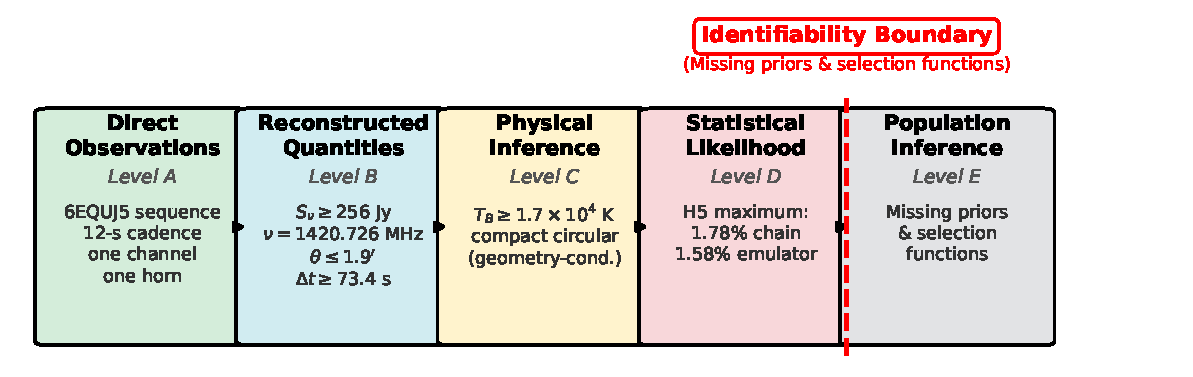
\includegraphics[width=0.95\textwidth]{fig1}
\caption{Provenance and identifiability architecture used in this analysis. Direct archival observations and documented historical results form the evidential base. Reconstructed quantities and deductive physical constraints can be evaluated where the surviving information is sufficient. Parameter likelihoods require a defined observation operator and selection function, while population posteriors additionally require defensible population priors. Progression to a higher inferential level is conditional on the information required at that level; it is not automatic.}
\label{fig:architecture}
\end{figure*}

\subsection{Direct Observations Versus Reconstruction}

The Big Ear archive is not a modern calibrated time--frequency data cube. The receiver sampled its channels at roughly 12-s cadence \citep{mendez2024}, and the event survives in the printout as the familiar ``6EQUJ5'' sequence in channel~2. Precise coordinates, corrected frequencies, and flux-density estimates therefore come from later calibration, beam modelling, and forensic reconstruction rather than directly from the original printout.

Those reconstructed values are useful, but they carry assumptions that the printout itself does not. We therefore treat them as reconstructed constraints rather than raw measurements and keep that distinction explicit throughout the analysis.

\subsection{Censored Quantities}

Three of the key reconstructed quantities are one-sided constraints.

The recovered flux density is a lower bound,
\[
\snu\geq256\pm63~{\rm Jy},
\]
under the adopted Arecibo~II calibration. Because the source position within the declination response is uncertain, it need not have crossed the beam maximum; an off-axis source would require a larger intrinsic flux to produce the recorded response. We therefore retain 256~Jy as a lower limit rather than a point estimate.

The source angular extent is bounded above,
\[
\theta\leq1.9\pm0.1~{\rm arcmin}.
\]
This limit enters the brightness-temperature calculation through the source solid angle. Within a chosen source geometry, the least restrictive lower bound follows from pairing the largest allowed solid angle with the smallest allowed flux. The sensitivity to the adopted brightness profile is treated in Section~\ref{sec:h3}.

The duration is likewise retained as a lower bound,
\[
\Delta t\geq73.4\pm0.5~{\rm s}.
\]
It refers to the beam-integrated duration of the recorded event, not directly to the time for which the source itself emitted.

\subsection{Selection Functions and Likelihood Identifiability}

For a set of competing hypotheses $H_i$, Bayesian model comparison requires
\begin{equation}
P(H_i\mid D)=
\frac{P(D\mid H_i)P(H_i)}
{\sum_j P(D\mid H_j)P(H_j)}.
\end{equation}

The likelihood also depends on how the observation was made. Schematically,
\begin{equation}
P(D\mid H_i)=
\int P(D\mid\vartheta,\mathcal{S})
P(\vartheta\mid H_i)\,d\vartheta,
\label{eq:general_likelihood}
\end{equation}
where $\vartheta$ denotes model parameters and $\mathcal{S}$ is the relevant selection function.

Here the selection function may include sensitivity, detection thresholds, false-alarm criteria, RFI excision, candidate-generation rules, temporal coverage, and rejection procedures. If those ingredients are unknown, observing time by itself does not determine the likelihood of a non-detection. Exposure and a verified null result are therefore different kinds of evidence.

When the selection information is missing, we leave the corresponding likelihood unidentified rather than supply an assumed threshold. That choice matters directly for the 2010--2014 Hobart archive and ultimately prevents a defensible five-way posterior.

%% ══════════════════════════════════════════════════════════════════════
%% SECTION 3
%% ══════════════════════════════════════════════════════════════════════

\section{Observational and Archival Evidence}
\label{sec:observations}

\subsection{Frozen Big Ear and Arecibo~II Constraints}

Our working observational vector comes from the Arecibo~II forensic reanalysis of the original Ohio SETI material \citep{mendez2025}. We froze that source to arXiv v1, dated 2025 August 14, in the project evidence manifest on 2026-08-23.

Any later journal revision of the reconstructed parameters would propagate into Sections~\ref{sec:h2}--\ref{sec:seldemo}. The Hobart donor archive was inventoried on 2026-08-25, followed by a donor-response round on 2026-08-29. Throughout the paper, one-sided quantities are kept as bounds rather than converted into point estimates.

\begin{figure*}[ht!]
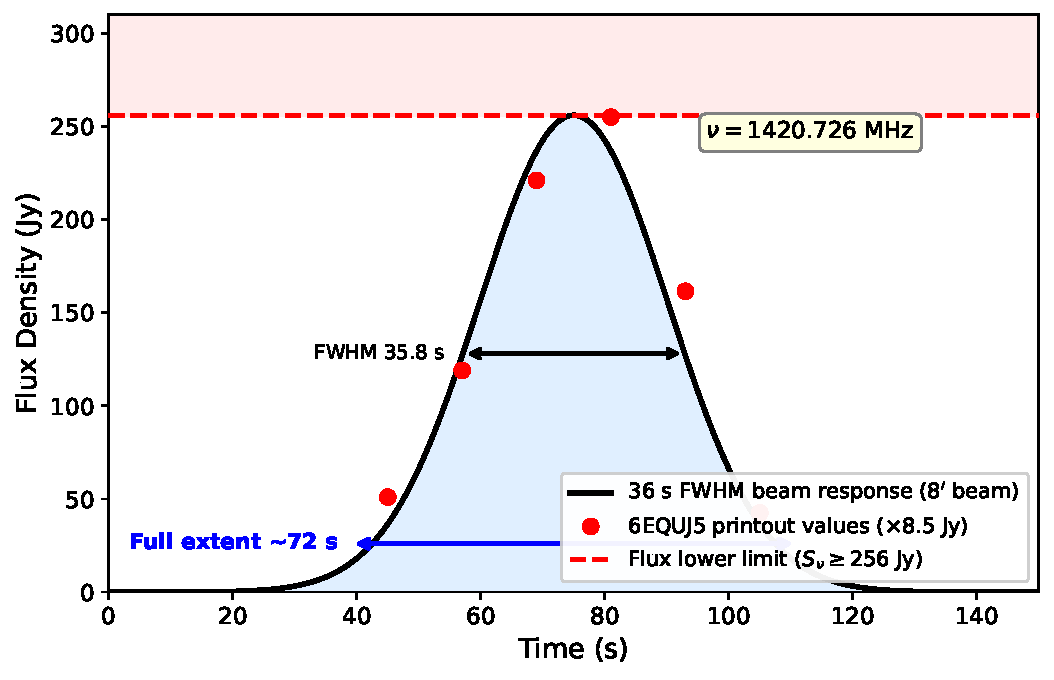
\includegraphics[width=0.45\textwidth]{fig2}
\caption{Frozen observational constraints used in the analysis. The 36-s FWHM beam response (8-arcmin beam at $\delta\simeq-27^\circ$) is schematic; red points show the recorded 6EQUJ5 printout values (decoded 6, 14, 26, 30, 19, 5$\sigma$) scaled by the 8.5-Jy channel noise at the 12-s receiver cadence. At S/N~$\simeq30$ the full detectable extent spans $\simeq72$--80~s, consistent with the recorded $6\times12$-s sequence. The 72~s is therefore the full detectable extent, not the FWHM. The flux-density constraint is explicitly treated as a lower limit. The frequency is fixed at the reconstructed topocentric value from the Arecibo~II analysis. The figure shows the structure of the observational constraints rather than implying an uncensored measurement of either flux or intrinsic duration.}
\label{fig:obs_constraints}
\end{figure*}

%% ----------------------------------------------------------------------
%% TABLE 1
%% Fixed-width columns keep the Limit and Units headers visually separate.
%% ----------------------------------------------------------------------
\begin{table*}[ht!]
\centering
\caption{Frozen observational evidence vector}
\label{tab:obs_vector}
\small
\setlength{\tabcolsep}{4pt}
\begin{tabular}{@{}
>{\raggedright\arraybackslash}p{0.31\textwidth}
>{\centering\arraybackslash}p{0.18\textwidth}
>{\centering\arraybackslash}p{0.06\textwidth}
>{\raggedright\arraybackslash}p{0.10\textwidth}
>{\raggedright\arraybackslash}p{0.23\textwidth}
@{}}
\hline Quantity & Value & Limit & Units & Source \\ \hline\hline
Observed frequency ($\nu$)
& $1420.726\pm0.005$ & --- & MHz & \citet{mendez2025}\\
Flux density ($\snu$)
& $256\pm63$ & $\geq$ & Jy & \citet{mendez2025}\\
Channel noise ($\sigma_{\rm ch}$)
& $8.5\pm2.1$ & --- & Jy & \citet{mendez2025}\\
Peak signal-to-noise ratio
& $30.1\pm0.4$ & --- & $\sigma$ & \citet{mendez2025}\\
Source angular extent ($\theta$)
& $1.9\pm0.1$ & $\leq$ & arcmin & \citet{mendez2025}\\
Transit duration ($\Delta t$)
& $73.4\pm0.5$ & $\geq$ & s & \citet{mendez2025}\\
Heliocentric velocity ($v_{\rm helio}$)
& $-84\pm1$ & --- & km\,s$^{-1}$ & \citet{mendez2025}\\
LSR velocity ($v_{\rm LSR}$)
& $-74\pm2$ & --- & km\,s$^{-1}$ & \citet{mendez2025}\\
R.A. (positive horn)
& $19^{\rm h}25^{\rm m}02^{\rm s}\pm3^{\rm s}$ & --- & J2000 & \citet{mendez2025}\\
R.A. (negative horn)
& $19^{\rm h}27^{\rm m}55^{\rm s}\pm3^{\rm s}$ & --- & J2000 & \citet{mendez2025}\\
Declination (both horns)
& $-26^\circ57'\pm20'$ & --- & J2000 & \citet{mendez2025}\\
\end{tabular}

\par {\small Censored quantities are retained as one-sided bounds; the ``Limit'' column indicates the sense of the bound, and ---\ marks quantities adopted as two-sided measurements. The transit duration is a lower bound on the observed beam-integrated event duration rather than a measurement of the intrinsic emission lifetime. All values are taken from the Arecibo~II reanalysis.}
\end{table*}

The event occupied a single receiver channel and changed strongly with time. Arecibo~II reconstructs a topocentric frequency of $1420.726\pm0.005$~MHz, corresponding to heliocentric and local-standard-of-rest velocities of about $-84\pm1$ and $-74\pm2$~km\,s$^{-1}$, respectively \citep{mendez2025}. We use these numbers as constraints on possible explanations, not as evidence for any one mechanism.

Figure~\ref{fig:obs_constraints} puts the transit timescale and flux limit on the same footing. The beam FWHM is about 36~s, whereas a source detected out to roughly $2.6\sigma$ on either side of the beam centre at S/N~$\simeq30$ remains visible for about 72~s, consistent with the recorded sequence. The Arecibo~II duration is still retained as a lower limit because the time recorded in the beam need not equal the source's intrinsic emission lifetime.

\subsection{Hobart 1998--1999}

The 1998--1999 Mount Pleasant campaign provides a comparatively clean follow-up constraint because both its sensitivity and its null result were published \citep{gray2002}. Six sessions of roughly 14~hr each gave about 82~hr on the Big Ear error boxes.

The search used a 2.5-MHz band divided into 4096 channels, giving approximately 610-Hz spacing. \citet{gray2002} reported a threshold near $5.9\sigma$ and a flux-density scale of about 18~Jy. Unlike the later archive discussed below, this campaign therefore supplies a documented non-detection with an explicit sensitivity scale.

That result can constrain models that predict frequent repetition, but the original reduction pipeline cannot now be reconstructed in full. We use the published non-detection as historical evidence and do not claim to have re-executed every step of the original search.

\subsection{Hobart 2010--2014}

A later Mount Pleasant campaign left a larger body of archival material. The surviving records preserve pointings, observing epochs, and exposure information, so they establish when the telescope was directed at the relevant sky positions.

What is missing is equally important. The archive does not preserve the detection thresholds, candidate-extraction rules, RFI masks, or candidate lists associated with the historical processing attributed to Bob Gray. The exposure record therefore cannot, by itself, establish a well-defined ``zero detections'' outcome.

This is a selection-function problem, not a statement about what physically occurred during the observations. With a documented threshold and candidate rule, the sessions could contribute a formal non-detection likelihood. Without them, treating the full campaign as a verified null would amount to reconstructing the historical search process by assumption. We therefore retain the 2010--2014 material as evidence of pointing and exposure but do not use it as a quantitative H5 null result.

%% ----------------------------------------------------------------------
%% Width budget: 0.11+0.24+0.20+0.18 = 0.73\textwidth of column text,
%% plus 8*\tabcolsep = 32pt of gutter. Well inside \textwidth, so the
%% class's automatic landscape fallback is never triggered.
%% ----------------------------------------------------------------------
\begin{table*}[ht!]
\centering
\caption{Archive and follow-up evidence status}
\label{tab:archive_status}
\begin{tabular}{>{\raggedright\arraybackslash}p{0.11\textwidth}>{\raggedright\arraybackslash}p{0.24\textwidth}>{\raggedright\arraybackslash}p{0.20\textwidth}>{\raggedright\arraybackslash}p{0.18\textwidth}}
\hline Dataset & Documented constraints & Missing elements & Inferential status \\ \hline\hline
Big Ear (1977)
& Signal sequence, transit morphology, channel information
& Complete modern raw time--frequency record
& Direct / reconstructed\\
VLA follow-up
& Published sensitivity and observing constraints
& Extended continuous time series
& Published constraint$^{a}$\\
Hobart (1998--1999)
& $\sim$82~hr, $5.9\sigma$, $\sim$18~Jy scale
& Historical raw reduction material
& Published non-detection$^{b}$\\
Hobart (2010--2014)
& Pointings, epochs, exposure
& Thresholds, candidate lists, selection rules
& Selection function unresolved\\
\end{tabular}

\par $^{a}$\citet{gray2001}.

\par $^{b}$\citet{gray2002}.
\par {\small The 2010--2014 records are not interpreted as a confirmed null result. Missing detection metadata prevent reconstruction of the corresponding empirical selection function.}
\end{table*}

%% ══════════════════════════════════════════════════════════════════════
%% SECTION 4
%% ══════════════════════════════════════════════════════════════════════

\section{H1 --- Instrumental or Radio-Frequency Interference Origin}
\label{sec:h1}

\subsection{Observed Characteristics Relevant to H1}

Any instrumental or radio-frequency interference explanation has to reproduce several features at once: the narrow spectral occupancy, the time-varying envelope, its approximate match to the telescope beam response, and the absence of a corresponding signal in the second horn.

Those features weigh against some mechanisms more strongly than others, but they do not define a probability distribution over the entire instrumental/RFI class. Ruling out H1 as a whole would require a much more complete account of receiver failure modes, terrestrial transmitters, sidelobe coupling, propagation, and the instrumental state of Big Ear at the time.

\subsection{Mechanism-Level Considerations}

Several mechanisms remain conceivable in principle. A receiver fault could create a large excursion in one channel, although it would also have to reproduce the multi-integration rise and fall of the observed sequence. Terrestrial signals might enter through sidelobes or other coupling paths, but their appearance would depend on transmitter position, frequency stability, propagation, and the telescope response. Reflections from aircraft or satellites add another set of geometric and Doppler constraints.

The Arecibo~II reanalysis \citep{mendez2025} gives several mechanism-level arguments, which we treat as constraints rather than a complete H1 likelihood. Its authors argue that the dual-horn configuration disfavors interference local to the telescope and that lunar reflection is inconsistent with the event geometry. Under the discrete, equiprobable amplitude-state model adopted by M\'endez et al. (2025), they also obtain the heuristic estimate $(1/32)^6\sim10^{-9}$ for a six-sample excursion of this form. That number is conditional on the assumed amplitude-state model and is not a probability for the full RFI hypothesis. The protected status of the 1420-MHz band, the documented absence of the relevant UHF television channels in Ohio in 1977, and the kinematics of geostationary and Molniya-type satellites further restrict specific terrestrial or near-Earth explanations. Solar and geomagnetic activity was also quiet, while the relevant solar-burst classes are poor matches in frequency or bandwidth. A later VLA search found no persistent narrowband point source at the locale \citep{gray2001}. These points narrow the mechanism space, but they still do not define a probability model over H1. The mechanism-level facts summarized here come from the cited Arecibo~II reanalysis and follow-up literature rather than being independently re-derived in this paper.

The surviving record also lacks the auxiliary monitoring needed to build a complete likelihood over these possibilities. Failure to identify a specific RFI mechanism should therefore not be read as evidence that the RFI probability is zero.

\subsection{Inferential Status}

For H1, the strongest statement supported by the frozen evidence is:
\begin{quote}
\emph{No specific instrumental or RFI mechanism in the frozen evidence set has been quantitatively demonstrated to reproduce the complete observed event.}
\end{quote}

The broader instrumental/RFI class remains unresolved. The available evidence constrains individual mechanisms, but it does not provide the model needed for a quantitative comparison with the other hypotheses.

%% ══════════════════════════════════════════════════════════════════════
%% SECTION 5
%% ══════════════════════════════════════════════════════════════════════

\section{H2 --- Cometary Origin}
\label{sec:h2}

\subsection{Geometric and Temporal Requirements}

A cometary explanation has two basic requirements: a plausible Solar System body must lie in the relevant beam at the event epoch, and its emission must match the observed spectral and temporal behaviour. The two objects proposed in this context are 266P/Christensen and 335P/Gibbs \citep{paris2017}.

The revised Arecibo~II reconstruction makes the test more restrictive. Its position is shifted by 7.25~arcmin relative to earlier estimates and the quoted error box is more than three times narrower \citep{mendez2025}. It also gives $1420.726\pm0.005$~MHz, corresponding to a heliocentric radial velocity of $-84\pm1$~km~s$^{-1}$. A cometary H\,I interpretation would instead track the comet's geocentric radial velocity at the event epoch, which can be obtained from the ephemeris.

Beam occupancy is only the first test. A viable comet candidate would also need the appropriate radial velocity and an emission process capable of matching the observed frequency and flux density.

\subsection{Geometric Exclusion from the Beam}
\label{sec:h2_ephem}

We generated independent geocentric ephemerides for both objects with JPL Horizons at 1977 August 16 03:16:06 UTC. At $\sim4$~AU, topocentric parallax is only $\sim2$~arcsec and is negligible compared with the degree-scale separations found here. We adopted the frozen M\'endez~II Table~4 J2000 horn positions: positive horn $19^{\rm h}25^{\rm m}02^{\rm s}\pm3^{\rm s}$, $-26^\circ57'18''\pm20'$; negative horn $19^{\rm h}27^{\rm m}55^{\rm s}\pm3^{\rm s}$, $-26^\circ57'13''\pm20'$. The printed positive-horn Galactic latitude ($b=-17.85$) was not used because an independent recomputation gives $b=-18.82$, a $0.97^\circ$ discrepancy; the other Table~4 Galactic-coordinate entries agree to within $0.03^\circ$.

At the event epoch, 266P/Christensen (JPL solution 2019-09-03; 539 observations from 2006--2014) is at RA $18^{\rm h}31^{\rm m}50.7^{\rm s}$, Dec $-27^\circ21.7'$, and $r=4.73$~AU. Relative to the positive horn it is displaced by 3191~s (53.2~min) in RA and $-24.3'$ in declination, corresponding to an exact on-sky separation of $11.8^\circ$; relative to the negative horn the offsets are 3364~s (56.1~min), $-24.4'$, and $12.5^\circ$. For 335P/Gibbs (JPL solution 2023-06-01; 430 observations from 2008--2023), the epoch position is RA $18^{\rm h}39^{\rm m}12.5^{\rm s}$, Dec $-29^\circ37.0'$, and $r=4.56$~AU. Its offsets are 2749~s (45.8~min) and $-159.7'$ from the positive horn ($10.4^\circ$ on-sky), and 2922~s (48.7~min) and $-159.8'$ from the negative horn ($11.0^\circ$ on-sky). These displacements are far larger than the adopted $\pm3$-s RA uncertainties and the $40'$ declination beam.

The formal $3\sigma$ ephemeris uncertainties (266P RSS $179''$; 335P RSS $10''$) are tiny compared with the measured offsets even if inflated by a factor of 100, although formal covariances do not capture every uncertainty in multi-decade back-integration with non-gravitational forces. The exclusion therefore depends on four explicit inputs: the event epoch, the adopted M\'endez~II horn coordinates and uncertainties, the stated Horizons solutions and observation arcs, and the direct geometric comparison with the horn error boxes. The resulting positions agree with the point-by-point rebuttal by members of the original Big Ear team \citep{naapo2017} to better than $1'$ and provide the geometric basis used here.

For 266P/Christensen, heliocentric distance supplies an additional physical constraint. At $r=4.73$~AU the comet was well beyond the range in which solar heating normally drives strong water-ice sublimation in short-period comets ($\lesssim2$--3~AU), although CO/CO$_2$-driven activity at larger distances is well documented \citep{gicquel2023}. Water-driven activity is therefore expected to be strongly suppressed at the event epoch; more volatile-driven activity is not excluded.

\subsection{Geometric, Kinematic, and Emission Constraints}

Even if a comet satisfied the beam geometry, other constraints would remain. Most importantly, no independently validated cometary H\,I emission mechanism has been demonstrated to reproduce a narrowband signal at the required $\geq256$-Jy flux density.

The candidate comets also move too slowly to explain the one-horn detection without an additional short-lived variability mechanism. Their Horizons rates are only $\sim11$--13~arcsec~hr$^{-1}$, corresponding to sub-arcsecond motion during the $\sim162$--173~s inter-horn interval, compared with an $8'\times40'$ beam. A slow comet crosses the meridian beam on essentially the same Earth-rotation timescale as a fixed celestial source, so the transit duration itself does not exclude it; the missing second-horn response is the relevant constraint.

There is also a methodological issue with the original cometary claim. \citet{paris2017} reported signal strengths in decibels rather than in janskys. That is non-standard for radio-astronomical flux calibration and complicates comparison with the Big Ear signal. We treat this as a limitation of the published measurement procedure rather than as an independent physical exclusion.

\subsection{Inferential Status}

The two proposed comet candidates can be set aside on geometric grounds:
\begin{quote}
\emph{266P/Christensen and 335P/Gibbs are incompatible with the reconstructed event geometry at the Wow! epoch. The broader cometary H\,I idea is not geometrically excluded, but no independently validated emission pathway has been shown to reproduce the full observed signal at the required flux density.}
\end{quote}

In the cross-hypothesis comparison, we therefore set aside the two named candidates while leaving the generic cometary-emission class unvalidated rather than geometrically ruled out.

%% ══════════════════════════════════════════════════════════════════════
%% SECTION 6
%% ══════════════════════════════════════════════════════════════════════

\section{H3 --- Interstellar H\,I Cloud and Non-Thermal Flare}
\label{sec:h3}

\subsection{Frozen Arecibo~II Constraints}

The Arecibo~II reconstruction supplies the main physical inputs for an interstellar H\,I interpretation \citep{mendez2025}: a lower bound on flux density, an upper bound on angular extent, and a frequency close to the 21-cm transition. The transient-amplification scenario considered here follows \citet{mendez2024}, who propose that a magnetar- or soft-gamma-repeater flare could briefly enhance the H\,I line in a cold interstellar cloud through stimulated maser or superradiant emission.

The relevant reconstructed constraints are
\begin{gather}
\snu\geq256\pm63~{\rm Jy},\nonumber\\
\theta\leq1.9\pm0.1~{\rm arcmin},\nonumber\\
\nu=1420.726\pm0.005~{\rm MHz}.
\end{gather}

The two inequalities are one-sided constraints, and the quoted uncertainties refer to the reconstruction rather than to symmetric measurements of the true source properties. M\'endez et al. obtain the flux density from $\snu={\rm SNR}\times\sigma_{\rm ch}$ with ${\rm SNR}=30.1\pm0.4$, where $\sigma_{\rm ch}$ is the per-channel noise of the transcribed record. The $\pm63$~Jy term is the resulting $1\sigma$ uncertainty, while the lower-limit sign reflects the possibility of additional declination-dependent beam attenuation and uncertainty in the noise calibration. The $1.9'$ source size is a deconvolved extent along the right-ascension drift direction, derived from a Gaussian fit to the transit profile assuming an $8'$ RA beam; its quoted $\pm0.1'$ uncertainty is the fit uncertainty. Big Ear provides no comparable size constraint in declination.

At $\delta\simeq-27^\circ$, the sidereal drift rate is about 13.4~arcsec~s$^{-1}$, so an $8'$ FWHM beam is crossed in roughly 36~s. The angular-size bound and the fitted duration $\Delta t\geq73.4\pm0.5$~s both come from the M\'endez~II Gaussian-profile fit, not simply from counting printout samples. The familiar $\simeq72$-s span is the observed duration of the six 12-s printout values, whereas the 73.4-s value is the beam-integrated duration inferred from the fit. The two are numerically close but represent different quantities; neither is the intrinsic emission lifetime. We use the nominal values $\snu=256$~Jy and $\theta=1.9'$ below and then examine the stated reconstruction and profile uncertainties explicitly.

\subsection{Brightness-Temperature Lower Bound}

For a source of specific intensity $I_\nu$ and solid angle $\Omega$,
\begin{equation}
\snu\simeq I_\nu\Omega.
\end{equation}

In the Rayleigh--Jeans limit,
\begin{equation}
I_\nu=
\frac{2k_{\rm B}\nu^2}{c^2}\tbeq.
\end{equation}

Combining the two gives
\begin{equation}
\tbeq=
\frac{\snu c^2}
{2k_{\rm B}\nu^2\Omega}.
\label{eq:tb}
\end{equation}

A flux density becomes a brightness temperature only after a source solid angle has been specified. Big Ear constrains the extent along the RA drift direction but not in declination, so the conversion necessarily depends on a source model. As a compact reference case, we take the measured RA extent to be the diameter of a circular uniform disk, a standard convention for brightness-temperature constraints on unresolved or marginally resolved radio sources \citep{condon2016}. This choice is also close to the compact-cloud picture discussed by M\'endez et al. \citep{mendez2025}. It is not an observed morphology: extending the source in declination increases the solid angle and weakens the temperature requirement.

For the circular model, the largest allowed solid angle is
\begin{equation}
\Omega_{\max}
=
\pi\left(\frac{\theta_{\max}}{2}\right)^2,
\end{equation}
with $\theta_{\max}=1.9$~arcmin $=5.527\times10^{-4}$~rad, giving
\[
\Omega_{\max}\simeq2.40\times10^{-7}~{\rm sr}.
\]

Using $\snu=256$~Jy as the lower-limit flux,
\begin{align}
\tbeq
&\geq
\frac{(256\times10^{-26})c^2}
{2k_{\rm B}\nu^2\Omega_{\max}}
\nonumber\\
&\gtrsim
1.72\times10^4~{\rm K}.
\label{eq:tb_bound}
\end{align}

Equation~(\ref{eq:tb_bound}) is the nominal result for the adopted circular profile. Within that model, a larger true flux or a smaller true source can only raise $\tbeq$. Pushing the quoted reconstruction uncertainties in the conservative direction, to $\snu=193$~Jy and $\theta=2.0'$, gives
\[
\tbeq\geq1.17\times10^4~{\rm K},
\]
about 30\% below the nominal value.

There is a separate uncertainty in how the fitted $1.9'$ size should be translated into solid angle. M\'endez~II obtains it from a Gaussian-profile fit (their ``maximum size ... assuming a beamwidth of 8 arcminutes''), which does not by itself establish that $1.9'$ should be treated as a uniform-disk diameter. If it is instead interpreted as a Gaussian FWHM, the solid angle increases by $1/\ln2\simeq1.44$. The corresponding bounds are $\tbeq\geq1.19\times10^4$~K for the nominal inputs and $\simeq0.81\times10^4$~K when the quoted flux and size uncertainties are also moved in the conservative direction. The nominal compact-source result lies above the usual WNM temperature range under either profile convention; the doubly conservative Gaussian case reaches its upper end.

\begin{figure*}[ht!]
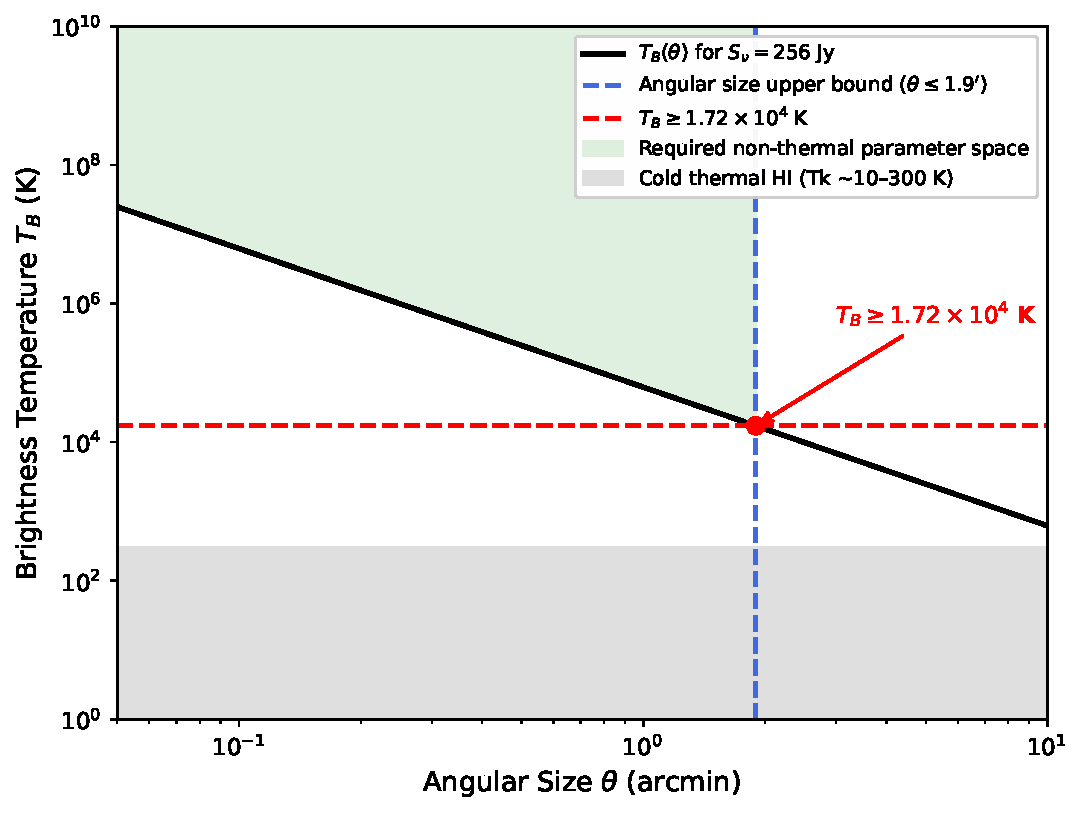
\includegraphics[width=0.45\textwidth]{fig3}
\caption{Brightness temperature as a function of angular source size for the conservative flux-density value $\snu=256$~Jy at $\nu=1420.726$~MHz. The angular-size constraint restricts the source to $\theta\leq1.9'$. At the largest allowed size, the corresponding nominal brightness temperature is $1.72\times10^4$~K, with a 1$\sigma$-propagated floor of $1.17\times10^4$~K. The figure represents a physical constraint conditional on the adopted circular-source geometry and does not encode a population probability for H3.}
\label{fig:h3_tb}
\end{figure*}

Figure~\ref{fig:h3_tb} shows the expected inverse-square dependence on angular size. Within the circular model, the least demanding temperature follows from the largest allowed source and the smallest allowed flux; a smaller or brighter source would raise the bound.

\subsection{Thermal Versus Non-Thermal Emission}

Cold neutral medium gas is typically tens to a few hundred kelvin, while the warm neutral medium reaches several thousand kelvin. For ordinary thermal 21-cm emission, the brightness temperature is limited by the excitation temperature and, in LTE, by the gas temperature.

Under the uniform-disk compact convention, both the nominal $1.72\times10^4$~K bound and the $1.17\times10^4$~K uncertainty floor lie above the usual WNM range. A compact source with that geometry would therefore require amplification beyond ordinary spontaneous thermal H\,I emission, such as stimulated or otherwise coherent emission. The profile calculation above shows, however, that this statement is conditional: in the doubly conservative Gaussian interpretation, the lower bound can approach the upper end of the WNM scale, and the unknown declination extent introduces a still larger geometric freedom.

This is a constraint on source physics, not a probability that H3 is correct. The occurrence rate, luminosity function, beaming distribution, pumping conditions, and spatial population of hypothetical transient H\,I amplification events are not known well enough to define a population prior. We therefore stop at the physical requirement rather than assigning $P({\rm H3}\mid D)$.

\subsection{Geometric Sensitivity: Declination-Elongated Sources}
\label{sec:h3_geometry}

The compact-source bound changes substantially if the emitter is extended in declination, the direction in which Big Ear had much poorer resolution.

Big Ear's half-power beamwidth was about $8'$ in RA and $40'$ in declination \citep{ehman1997,mendez2024}. Because the Wow! event was seen only once, there is no neighbouring declination scan from which to recover the source's north--south extent. The transit profile therefore constrains the size along the drift direction but leaves the declination extent unresolved within the much broader beam.

The reference circular model assigns a solid angle $\Omega_{\rm circ}=\pi(\theta_{\rm RA}/2)^2$ with $\theta_{\rm RA}=1.9'$ and hence $\Omega_{\rm circ}\simeq2.40\times10^{-7}$~sr. For a filament or sheet with the same RA width but a declination extent $\theta_{\rm Dec}$,
\begin{equation}
\Omega_{\rm elong}
=
\pi\left(\frac{\theta_{\rm RA}}{2}\right)
\left(\frac{\theta_{\rm Dec}}{2}\right),
\label{eq:omega_elong}
\end{equation}
so Equation~(\ref{eq:tb}) gives
\begin{equation}
\tbeq^{\rm (elong)}
=
\tbeq^{\rm (circ)}\times\frac{\theta_{\rm RA}}{\theta_{\rm Dec}}.
\label{eq:tb_elong}
\end{equation}

A source filling the full $\sim40'$ declination beam would therefore have about 21 times the solid angle of the circular reference case. The resulting brightness temperatures are
\begin{align}
\tbeq^{\rm (elong,\,nom)}
&\simeq
\frac{1.72\times10^4}{21}
\simeq
820~{\rm K},
\nonumber\\
\tbeq^{\rm (elong,\,floor)}
&\simeq
\frac{1.17\times10^4}{20}
\simeq
585~{\rm K}.
\label{eq:tb_elong_values}
\end{align}

For context, the WNM has characteristic kinetic temperatures of roughly 5000--8000~K, while the CNM is typically about 50--200~K \citep{wolfire2003}. The source need not fill the entire $40'$ beam to enter the WNM range. In the uniform-disk scaling, $\theta_{\rm Dec}\gtrsim4.09'$ lowers the nominal bound below 8000~K, and $\theta_{\rm Dec}\gtrsim6.54'$ lowers it below 5000~K. Under the Gaussian-profile convention these thresholds become $\gtrsim2.83'$ and $\gtrsim4.53'$, respectively.

The compact-source non-thermal requirement is therefore not geometry-independent. A nearly circular source demands a brightness temperature above the ordinary thermal phases of neutral H\,I, whereas a filament elongated mainly in declination can bring the requirement into the WNM range. We keep the circular calculation as the compact reference case, but the unconstrained north--south extent remains a real systematic uncertainty.

\subsection{HI4PI Check at the Event Velocity}
\label{sec:hi4pi}

The persistent-filament version of H3 can be tested against the HI4PI all-sky H\,I survey \citep{hi4pi2016}. We extracted spectra at the reconstructed positive- and negative-horn positions ($l\simeq11.62$, $b\simeq-18.82$ and $l\simeq11.87$, $b\simeq-19.42$; nearest-pixel separations 1.4 and 1.0~arcmin) and at declination offsets of $\pm20'$ and $\pm40'$ along both horn meridians. HI4PI has a $16.2'$ beam and 1.29~km\,s$^{-1}$ channels. Across $V_{\rm LSR}=-76$ to $-72$~km\,s$^{-1}$, centred on the Arecibo~II value of $-74\pm2$~km\,s$^{-1}$, all ten sampled spectra remain at or below 0.10~K in absolute value per channel, with local rms values of 0.01--0.05~K. The extracted values and reproduction script are listed in Section~\ref{sec:availability}. As a wider check, all 824 HI4PI pixels within $45'$ of either horn---covering both $40'$ declination beams and the coordinate uncertainties---remain below 1~K in the same velocity window, with a maximum of 0.15~K. HI4PI uses radio-definition LSRK velocities, while the Arecibo~II value is a kinematic-LSR velocity from the same solar-motion correction family; sub-km\,s$^{-1}$ frame differences are small compared with the 4~km\,s$^{-1}$ comparison window.

To compare the survey with the Wow! reconstruction, we model the source as a uniform-brightness ellipse with fixed RA width $1.9'$ and a free declination extent, and compute its overlap with the $16.2'$ Gaussian HI4PI beam. For source solid angle $\Omega_{\rm src}$ and peak-normalized beam response $P$,
\begin{equation}
T_{\rm meas} =
\frac{\snu c^2}{2k_{\rm B}\nu^2\Omega_{\rm src}}\,
\frac{\int_{\rm source} P\,d\Omega}{\Omega_{\rm beam}}
\times f_{\rm ch},
\label{eq:hi4pi_coupling}
\end{equation}
where the channel-share factor satisfies $f_{\rm ch}\leq1$ ($f_{\rm ch}=1$ for an unresolved narrow line and $\simeq0.61$ for a line filling the Big Ear channel).

For a line no broader than one HI4PI channel, the expected central-beam brightness is $\simeq163$~K for the compact finite-width model ($\simeq164$~K in the point-source limit), about 160~K for the $4$--$6.5'$ elongations that reach WNM temperatures, about 130~K at $20'$, and about 84~K for a filament filling the full $40'$ beam. The Big Ear channel width is about 2.11~km\,s$^{-1}$, compared with 1.29~km\,s$^{-1}$ for HI4PI, so channel averaging can change the narrow-line prediction only by a factor of order unity; it cannot bridge the gap between tens to hundreds of kelvin and the observed $\leq0.10$~K. A persistent source at the event velocity is therefore excluded across the tested elongations.

The spectral width provides a separate check. At 5000--8000~K, an ordinary thermal H\,I line would span roughly seven to nine 10-kHz Big Ear channels rather than one. A line peaking at 256~Jy in the detected channel would place about 240~Jy in each immediately adjacent channel, far above the $\sim8.5$~Jy channel noise, yet the event occupies only one channel. Within the geometries considered here, the remaining H3 interpretation is therefore transient and non-thermal. The HI4PI comparison concerns the persistent-filament alternative rather than the flare model of \citet{mendez2024}: it constrains persistent emission at the sampled velocity in a later survey epoch, not the source at the moment of the 1977 transient.

\begin{figure*}[ht!]
\centering
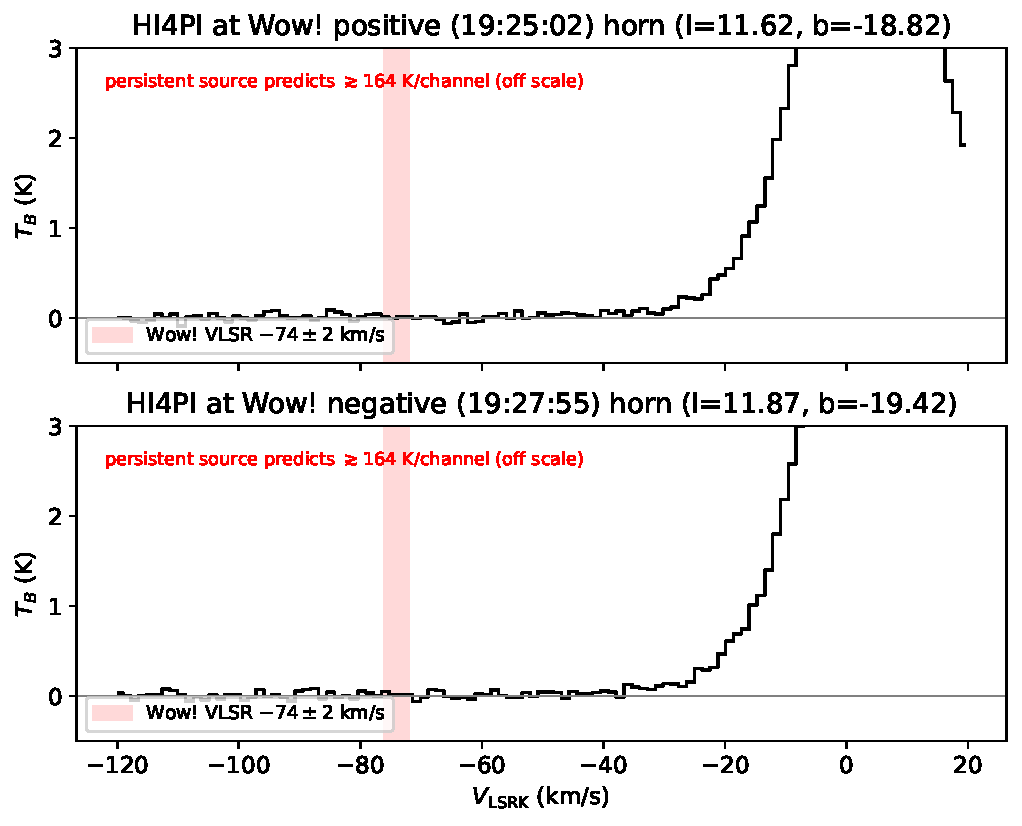
\includegraphics[width=0.85\textwidth]{fig4}
\caption{HI4PI spectra (16.2$'$ beam, 1.29~km\,s$^{-1}$ channels) at the Wow! positive and negative horn positions across the event velocity. The red band marks VLSR $-74\pm2$~km\,s$^{-1}$; measured brightness in the band is $<0.1$~K per channel (rms $\simeq0.04$~K) at both positions. A persistent compact source at the Wow! flux level would appear at $\gtrsim164$~K per channel (point-source limit); elongated morphologies dilute this across beams but remain excluded (Sec.~\ref{sec:hi4pi}).}
\label{fig:hi4pi}
\end{figure*}

%% ══════════════════════════════════════════════════════════════════════
%% SECTION 7
%% ══════════════════════════════════════════════════════════════════════

\section{H4 --- Artificial Power-Beam Leakage}
\label{sec:h4}

\subsection{Conditional Radiometric Requirement}

If the signal were leakage from a highly directional power-beaming system, the required transmitter strength can be written in terms of isotropic-equivalent radiated power (EIRP). The received spectral flux density is
\begin{equation}
\snu=
\frac{{\rm EIRP}}
{4\pi D^2\Delta\nu},
\label{eq:eirp}
\end{equation}
where $D$ is the source distance and $\Delta\nu$ is the effective emission bandwidth.

The bandwidth is not measured. Big Ear recorded the signal in one 10-kHz channel, so $\Delta\nu\leq10$~kHz but could be much smaller. Narrow emission is also plausible for high-gain microwave amplifiers, which can operate with small fractional bandwidths \citep{benford2025}. The radiometric requirement must therefore remain conditional on an assumed $\Delta\nu$:
\begin{equation}
\begin{split}
{\rm EIRP}_{\rm req}(D,\Delta\nu)
&=
4\pi D^2\,\snu\,\Delta\nu \\
&\simeq
3.06\times10^{14}
\left(\frac{D}{1~{\rm pc}}\right)^2 \\
&\quad\times
\left(\frac{\Delta\nu}{10~{\rm kHz}}\right)
\left(\frac{\snu}{256~{\rm Jy}}\right)
~{\rm W},
\end{split}
\label{eq:eirp_req}
\end{equation}
using the lower-limit flux density $\snu=256$~Jy. If the signal fills the full 10-kHz channel, the received band-integrated flux is at least $2.56\times10^{-20}$~W~m$^{-2}$. Equation~(\ref{eq:eirp_req}) scales linearly with bandwidth and quadratically with distance. The 10-kHz case is therefore the largest EIRP compatible with a single-channel interpretation at a fixed distance; a narrower signal requires proportionally less power. Because neither $D$ nor $\Delta\nu$ is measured, H4 is described by a family of radiometric requirements rather than a single transmitter power.

\begin{table}[ht!]
\centering
\caption{Conditional EIRP requirement (W) as a function of assumed source distance and emission bandwidth, from Equation~(\ref{eq:eirp_req}) with $\snu=256$~Jy}
\label{tab:eirp}
\begin{tabular}{lccc}
\hline Distance & $\Delta\nu=1$~Hz & $\Delta\nu=1$~kHz & $\Delta\nu=10$~kHz \\ \hline\hline
100~AU (Solar System) & $7.2\times10^{3}$ & $7.2\times10^{6}$ & $7.2\times10^{7}$ \\
1.3~pc & $5.2\times10^{10}$ & $5.2\times10^{13}$ & $5.2\times10^{14}$ \\
10~pc & $3.1\times10^{12}$ & $3.1\times10^{15}$ & $3.1\times10^{16}$ \\
100~pc & $3.1\times10^{14}$ & $3.1\times10^{17}$ & $3.1\times10^{18}$ \\
1~kpc & $3.1\times10^{16}$ & $3.1\times10^{19}$ & $3.1\times10^{20}$ \\
\end{tabular}

\par {\small All entries scale linearly with the assumed bandwidth and with the adopted flux-density lower bound. The 10-kHz column assumes the emission fills the recorded channel and therefore represents the largest requirement consistent with the single-channel record, not a lower bound.}
\end{table}

Table~\ref{tab:eirp} gives the corresponding values. Cost-optimized interstellar beacon concepts can reach ${\rm EIRP}\sim10^{17}$~W at gigahertz frequencies and use dwell times of order 10--100~s \citep{benford2010,benford2021}. On that scale, a channel-filling 10-kHz Wow!-like signal is comparable only for a relatively nearby source, roughly $D\lesssim10$--30~pc; a narrower signal could be seen from farther away at the same EIRP. At 1~kpc, the channel-filling requirement rises to $3.1\times10^{20}$~W. Solar-System distances are radiometrically easy by comparison, which is why later targeted searches with substantially lower flux limits \citep[e.g.][]{perez2022} are more relevant to a nearby-transmitter version of H4. These numbers are scaling relations rather than estimates of a real transmitter because the source distance and emission geometry are both unknown.

For antenna gain $G$, the physical transmitter power is approximately
\[
P_t={\rm EIRP}/G.
\]
The gain depends on aperture, illumination efficiency, and wavelength. A large aperture can provide very high directivity at 1.42~GHz, but the surviving evidence does not justify choosing a specific transmitter design.

\subsection{The Frequency Coincidence}

Radiometry alone does not rule out accidental power-beam leakage, but the observing frequency is not an obvious engineering optimum for such a system. Beam divergence, atmospheric and interstellar transmission, and power-generation efficiency generally favour higher microwave frequencies---roughly a few to tens of GHz in the engineering literature considered here---or optical/near-infrared wavelengths for light-sail concepts \citep{benford2010}. At 21~cm, a given beam solid angle also requires a larger aperture than at shorter wavelengths, and propagation along sufficiently H\,I-rich sightlines can introduce line-specific absorption or stimulated-emission effects. None of these points is a universal prohibition, but they make 1420~MHz a less obvious choice for energy transfer.

The same frequency has a very different history in SETI. Since \citet{cocconi1959}, the H\,I line has been treated as a natural Schelling point for intentional communication, and \citet{oliver1971} later extended that idea to the 1.42--1.66~GHz ``water hole.'' Benford's power-beaming arguments favour microwaves in general \citep{benford2021}, but they do not specifically select the H\,I line.

A simple frequency-window calculation illustrates the dependence on assumptions. Big Ear covered only about 500~kHz instantaneously (rest-frame nominal centre 1420.4056~MHz; GSR-tracked centre $\approx1420.491$~MHz at the event, spanning 1420.246--1420.736~MHz). If one adopts a uniform transmitter-frequency prior over 1--100~GHz, the fraction of that interval falling inside the Big Ear window is $\sim5\times10^{-6}$. A log-uniform prior over the same range gives $\sim7.6\times10^{-5}$, about 15 times larger. These numbers are not probabilities that H4 is correct and are not used as likelihood penalties.

The calculation also has an important selection effect: Big Ear was deliberately observing a narrow band near the H\,I line. Conditional on an event having been detected by that experiment, finding it in the monitored band is partly a consequence of the observing setup. A proper population calculation would need to model the transmitter-frequency distribution jointly with the telescope selection function. We therefore keep the 1420-MHz coincidence as a conditional illustration under an adopted frequency prior, not as independent empirical evidence against H4.

\subsection{Population-Level Limitation}

The radiometric calculation tells us what a transmitter would need to deliver at a chosen distance and bandwidth. It does not tell us how common such systems are, where they are located, how often they operate, or how often their beams intersect Earth. Those missing population quantities prevent a posterior probability for H4.

H4 is therefore retained as a conditional feasibility calculation rather than promoted to a probabilistic explanation.

%% ══════════════════════════════════════════════════════════════════════
%% SECTION 8
%% ══════════════════════════════════════════════════════════════════════

\section{H5 --- Stochastic Repeating ETI Beacon}
\label{sec:h5}

\subsection{The Kipping--Gray Stochastic Model}

\citet{kipping2022} modelled the Wow! signal as a possible member of a stochastic repeating process. Event start times follow a homogeneous Poisson process with rate $\lambda$, and each event lasts for a duration $T$.

For an interval $\Delta t$, the expected number of event starts is
\begin{equation}
\mu=\lambda\Delta t,
\end{equation}
and the number of events $k$ follows
\begin{equation}
P(k\mid\mu)=
\frac{\mu^k e^{-\mu}}{k!}.
\label{eq:poisson}
\end{equation}

The count process is only part of the problem. A simulated event must also overlap the relevant Big Ear observing window and satisfy the two-horn timing constraint. The Kipping--Gray likelihood therefore combines the Poisson process with the actual observing schedule and horn geometry.

The result is a likelihood surface over $(\lambda,T)$, not a probability that H5 is true. We therefore quote the maximum likelihood on that surface. We avoid the phrase ``MAP likelihood'': a maximum a posteriori estimate depends on a prior, even though the flat log-space priors used in the released chains place the posterior mode at the same grid point. None of the percentages below should be read as $P({\rm H5}\mid D)$.

\subsection{Verification against the Published Implementation}
\label{sec:h5_verify}

The public Kipping--Gray release makes the published result directly checkable \citep{kipping2022code}. Their Fortran program \citep[{\tt wow.f90};][]{kipping2022code} evaluates a $150\times160$ grid, logarithmically spaced in $T\in[72~{\rm s},e^{-1}~{\rm d}]$ and $\lambda\in[e^{-4},e^2]~{\rm day}^{-1}$, with a hard event-count truncation at $\kmax=100$. At each grid point the code Monte-Carlo samples Poisson event trains over the 2673-day baseline containing the 90 documented Big Ear observing days. A hit must overlap the 72-s primary-horn window without producing an incompatible response 162~s later in the second horn. The released chains then apply three tiers of constraints: OSU alone, OSU plus the published 1998--1999 Hobart non-detection, and the full set including META and the Allen Telescope Array \citep{harp2020}.

Taking the maximum of the log-likelihood column in each released chain reproduces the published values exactly: $32.3\%$ for OSU, $3.3\%$ for OSU$+$Hobart, and $1.78\%$ for ALL. The all-constraints maximum is therefore verified against the authors' own release. The progression $32.3\%\rightarrow3.3\%\rightarrow1.78\%$ also makes clear how strongly the H5 parameter likelihood responds to the addition of follow-up searches and their selection functions.

\subsection{Independent Analytic Emulator}
\label{sec:h5_emulator}

We also built an independent analytic emulator as a cross-check. It evaluates the probability of exactly one Wow-like hit day and no other recognizable hit days over the same 2673-day baseline, summing Poisson event counts up to an explicit $\kmax$. The emulator uses the same 90 observing days, 72-s windows, and 162-s horn separation, while pooling 192~hr (8~d) of follow-up into a factor $\exp(-\lambda T_{\rm fu})$.

This construction is related to, but not identical with, the published pipeline. The original code samples event times explicitly, defines the conditioning event through its per-day hit logic, and applies follow-up constraints campaign by campaign. Those differences matter for the absolute scale: the emulator's no-follow-up maximum is $5.6\%$, compared with $32.3\%$ for the published OSU chain. We therefore use the emulator only for relative comparisons in which its own conventions are held fixed.

With $\kmax=100$, the emulator peaks at $\simeq0.8\%$. The result converges to $1.58\%$ for $\kmax\geq500$, and an untruncated Monte Carlo evaluation of the same estimator also gives $1.58\%$ (Figure~\ref{fig:h5_convergence}). The factor-of-two sensitivity at low truncation is a property of the emulator, not of the verified published value. The code used for the emulator, the released-chain check, and the selection-function calculation below is included in the reproducibility package described in Section~\ref{sec:availability}.

\begin{figure*}[ht!]
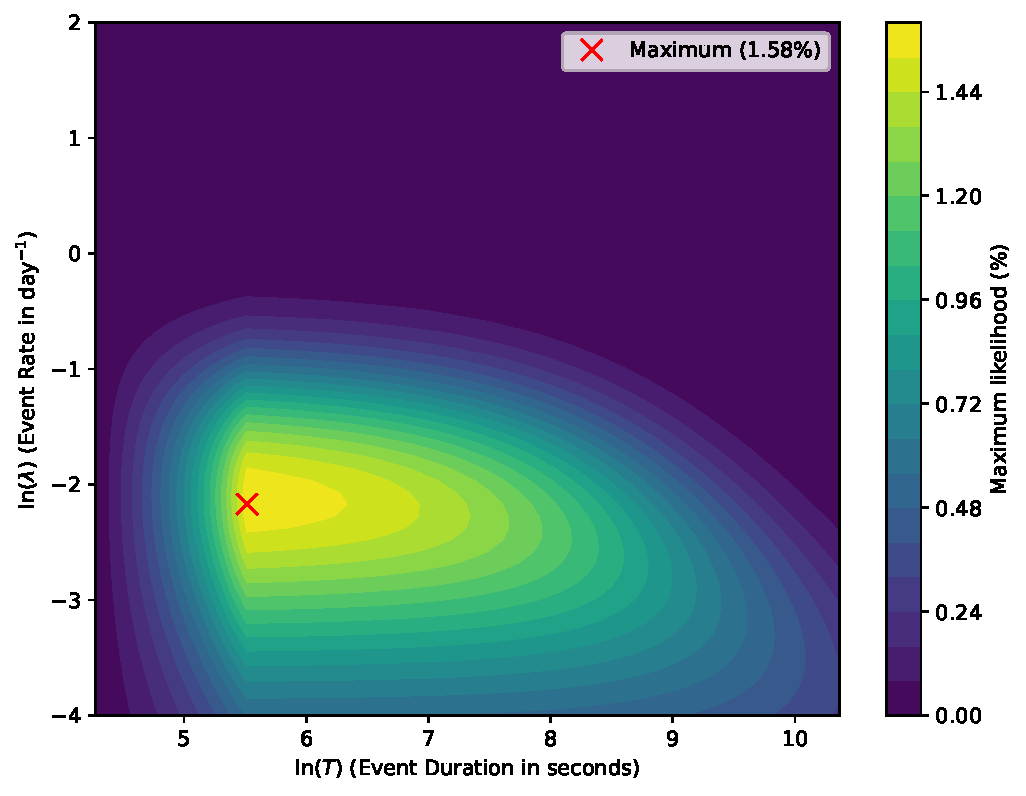
\includegraphics[width=0.45\textwidth]{fig5}
\caption{Independent analytic emulator (Section~\ref{sec:h5_emulator}) of the H5 stochastic-repeater parameter likelihood in $(\ln T,\ln\lambda)$ space, including the pooled 192-hr follow-up non-detection factor. The displayed quantity is a parameter likelihood associated with the stochastic-repeater model, not a posterior probability that H5 is correct; its cross is the maximum of the emulator likelihood. The peak location depends on the numerical grid used for the reconstruction.}
\label{fig:h5_likelihood}
\end{figure*}

\begin{figure*}[ht!]
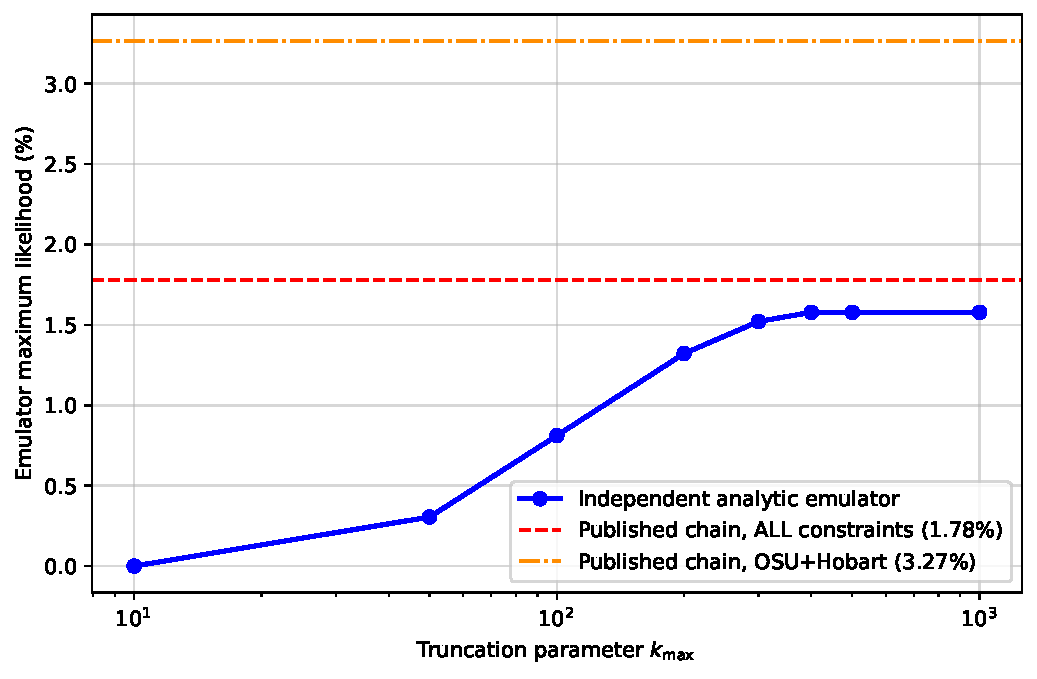
\includegraphics[width=0.45\textwidth]{fig6}
\caption{Convergence diagnostic for the independent analytic emulator of the H5 calculation. The figure compares the emulator maximum likelihood as $\kmax$ is increased, with the pooled 192-hr follow-up non-detection factor applied. Horizontal reference lines show the maximum likelihoods recomputed from the released published chains (OSU$+$Hobart: $3.3\%$; ALL: $1.78\%$). The purpose of the plot is to diagnose the emulator's numerical sensitivity to truncation, not to characterize the published result as a probability or to claim a revised hypothesis posterior.}
\label{fig:h5_convergence}
\end{figure*}

Figure~\ref{fig:h5_likelihood} shows the emulator likelihood surface, while Figure~\ref{fig:h5_convergence} shows its dependence on the event-count truncation. The finite sum approaches a stable value at large $\kmax$, consistent with the untruncated Monte Carlo check.

\begin{table}[ht!]
\centering
\caption{Emulator maxima, pipelines, and conditioning.}
\label{tab:emulator_map}
\setlength{\tabcolsep}{4pt}
\begin{tabular}{@{}l l>{\raggedright\arraybackslash}p{0.52\columnwidth}@{}}
\hline Maximum & Pipeline & Conditions \\ \hline\hline
$5.62\%$ & emulator & no follow-up (OSU-only) \\
$2.52\%$ & emulator & S1 scenario on Hobart 2010--14 upper-limit span \\
$1.58\%$ & emulator & pooled 192-hr follow-up \\
\hline
\end{tabular}
\par {\small The three emulator maxima differ only in follow-up conditioning and are not interchangeable with the published-chain maxima ($32.3\%$/$3.3\%$/$1.78\%$).}
\end{table}

\begin{table*}[ht!]
\centering
\caption{Verification and independent numerical characterization of the H5 calculation. The first three rows are recomputed maxima of the log-likelihood column in the released published chain files \citep{kipping2022code} and reproduce the published values; they are verifications, not independent reimplementations. The lower three rows come from the independent analytic emulator of Section~\ref{sec:h5_emulator}, whose conditioning and follow-up modeling differ from the published pipeline (see text); its absolute scale is therefore not directly comparable to the chain values, and it is used only for controlled relative comparisons. All values are parameter-likelihood maxima for the stochastic-repeater model, not posterior probabilities for H5.}
\label{tab:h5_recon}
\small
\setlength{\tabcolsep}{4pt}
\begin{tabular}{@{}lccc>{\raggedright\arraybackslash}p{0.24\textwidth}@{}}
\toprule
Implementation & Constraints & Truncation & Maximum likelihood & Interpretation \\
\midrule
Published chain (released) & OSU (1977 only) & $\kmax=100$ & $32.3\%$ & Verified from released chain \\
Published chain (released) & OSU$+$Hobart (1998--99) & $\kmax=100$ & $3.3\%$ & Verified from released chain \\
Published chain (released) & OSU$+$Hobart$+$META$+$ATA & $\kmax=100$ & $1.78\%$ & Verified from released chain \\
Independent analytic emulator & Pooled 192-hr follow-up & $\kmax=100$ & $\simeq0.8\%$ & Truncation-sensitive regime \\
Independent analytic emulator & Pooled 192-hr follow-up & $\kmax\geq500$ & $1.58\%$ & Converged emulator value \\
Independent Monte Carlo evaluation & Pooled 192-hr follow-up & Untruncated & $1.58\%$ & Cross-check of emulator \\
\bottomrule
\end{tabular}
\end{table*}

Table~\ref{tab:h5_recon} keeps the two numerical exercises separate. The published maxima are direct checks of the released chains. The emulator is an independent approximation with different conditioning and follow-up treatment, and its residual sensitivity to $\kmax$ is shown in Figure~\ref{fig:h5_convergence}. Neither set of values is a posterior probability for H5.

\subsection{2010--2014 Hobart Selection Function}

The later Hobart observations cannot simply be inserted into the likelihood as an exposure multiplied by a non-detection factor. That step would require knowing the probability that an event of the relevant type and strength would have been recognized during each observing interval.

The surviving 2010--2014 archive establishes pointings and exposure, but it does not preserve the historical threshold, candidate-generation procedure, false-alarm criterion, or candidate-outcome catalogue. The probability of recognizing an H5 event in those data is therefore not recoverable from the archive.

This does not mean that the campaign detected no candidates. It means that the records needed to define a quantitative null likelihood are missing. Treating the campaign as zero detections would insert an unverified selection function and could artificially suppress the inferred repetition rate. We therefore retain the archive as evidence of historical exposure and observing geometry, but not as a quantitative H5 null result.

\subsection{A Demonstrative Selection-Function Calculation}
\label{sec:seldemo}

The effect of the missing selection function can still be illustrated. The archive contains eleven 2010--2014 sessions at the Wow! locale with a summed first-to-last-spectrum span of $114.1$~h, or $T_{\rm H}=4.75$~d. These spans are upper limits on usable observing time.

We compare two limiting treatments, without assigning them equal prior weight. Under S1 (\emph{transparent}), every Wow-like event---a $\geq72$-s, high-flux narrowband transient in the tracked beam and band---is assumed to have been recognized, so the absence of a recognized event contributes $\exp(-\lambda T_{\rm H})$. Under S2 (\emph{opaque}), the missing threshold and candidate-selection metadata are taken to make the archive statistically uninformative, so the likelihood is unchanged. At fixed $(T,\lambda)$,
\[
\frac{L_{\rm S1}}{L_{\rm S2}}=\exp(-\lambda T_{\rm H}).
\]

This is only an illustrative convention. Treating the entire first-to-last-spectrum span as usable time can overstate the exposure, while ignoring events that begin before a session and continue into it understates the detectable start-time interval by up to a duration $T$ for each window. The two approximations therefore act in opposite directions, so $\exp(-\lambda T_{\rm H})$ is not a rigorous bound on the true penalty.

Figure~\ref{fig:hobart_selection} shows the ratio across the emulator's rate range. At its OSU-only maximum-likelihood rate, $\lambda^\ast=0.17~{\rm day}^{-1}$, the ratio is $0.44$; at $\lambda=1~{\rm day}^{-1}$ it is $8.7\times10^{-3}$; and for $\lambda\gtrsim5~{\rm day}^{-1}$ it falls below $10^{-10}$. Holding the emulator conventions fixed, S1 lowers the maximum from $5.62\%$ to $2.52\%$, a 2.2-fold reduction. Integrating over the adopted flat $(\ln T,\ln\lambda)$ grid gives a grid-integrated likelihood ratio of $0.65$ within that emulator and parameter domain. The $114.1$-h span used in S1 remains an upper limit on usable time.

The published chains provide a useful scale comparison, but not a calibration of the later archive. Adding the documented 1998--1999 Hobart non-detection moves the published maximum from $32.3\%$ to $3.3\%$ under its own selection function. Because the later campaign has a comparable amount of on-source time, an update of similar size could occur if its sensitivity and selection properties were also similar. Those properties are precisely what the surviving 2010--2014 archive does not preserve. The point of the exercise is therefore not to claim a particular update, but to show how strongly that update depends on assumptions about the missing selection function.

\begin{figure}[ht!]
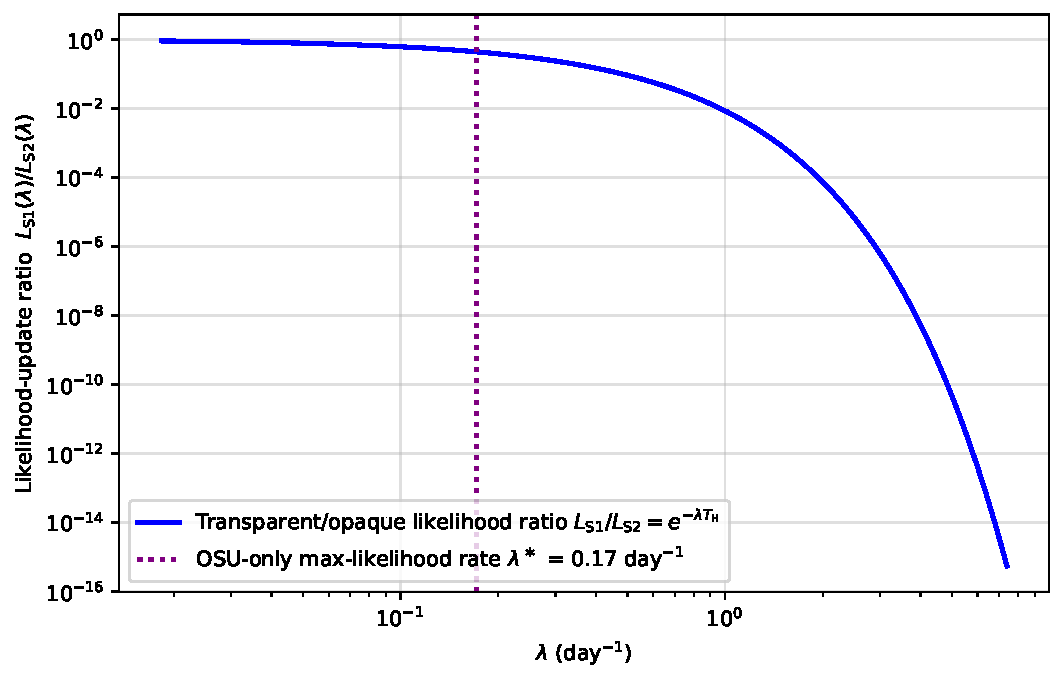
\includegraphics[width=0.45\textwidth]{fig7}
\caption{Selection-function dependence of the 2010--2014 Hobart likelihood update. The plotted quantity is the transparent-to-opaque likelihood ratio, $L_{\rm S1}/L_{\rm S2}=\exp(-\lambda T_{\rm H})$, for $T_{\rm H}=4.75$~d. S1 treats the $114.1$-h span as an effective non-detection, whereas S2 applies no quantitative constraint. The vertical line marks the OSU-only maximum-likelihood rate of the independent analytic emulator. The two limiting treatments demonstrate why the unresolved 2010--2014 selection function is not included in the quantitative H5 likelihood.}
\label{fig:hobart_selection}
\end{figure}

% FIGURE-ASSET NOTE: the external fig7.pdf legend currently uses the shorthand
% "S1 -> S2 update ratio". If the figure is regenerated, replace that legend
% with "Transparent/opaque likelihood ratio L_S1/L_S2 = exp(-lambda T_H)"
% to match the axis and caption exactly.

\subsection{Bayesian Marginalization over the Unknown Threshold}
\label{sec:h5_bayes_marg}

The binary S1/S2 comparison is only a limiting exercise. A more general treatment would regard the unknown historical detection threshold $S_{\rm th}$ as a nuisance parameter and marginalize over it.

For the Hobart 2010--2014 data,
\begin{equation}
P(D_{\rm H}\mid\lambda,T)
=
\int_0^\infty
P(D_{\rm H}\mid\lambda,T,S_{\rm th})\,
p(S_{\rm th})\,
dS_{\rm th},
\label{eq:marg_sth}
\end{equation}
where $P(D_{\rm H}\mid\lambda,T,S_{\rm th})$ is the likelihood conditional on a specified threshold. For a sharp threshold model,
\begin{equation}
P(D_{\rm H}\mid\lambda,T,S_{\rm th})
=
\begin{cases}
\exp(-\lambda\,T_H) \quad & \text{if } S_{\rm th}\leq S_{\rm Wow},\\
1 \quad & \text{if } S_{\rm th}>S_{\rm Wow},
\end{cases}
\label{eq:cond_sth}
\end{equation}
with $T_H=4.75$~d and $S_{\rm Wow}\geq256$~Jy. The first branch corresponds to S1 and the second to S2.

One possible scale prior is log-uniform, $p(S_{\rm th})\propto1/S_{\rm th}$ on $[S_{\min},S_{\max}]$. This is a modelling choice, not a uniquely determined prior, and the result depends on the adopted bounds. For $S_{\min}<S_{\rm Wow}<S_{\max}$,
\begin{equation}
P(D_{\rm H}\mid\lambda,T)
=
\frac{
\ln(S_{\rm Wow}/S_{\min})\,e^{-\lambda T_H}
+\ln(S_{\max}/S_{\rm Wow})
}
{\ln(S_{\max}/S_{\min})},
\label{eq:marg_result}
\end{equation}
which interpolates smoothly between the transparent limit $e^{-\lambda T_H}$ and the opaque limit of unity.

This kind of selection-function treatment is standard in modern transient population work. CHIME/FRB uses large synthetic-injection campaigns to characterize its selection function and marginalizes over remaining calibration uncertainties \citep{amiri2021}. Gravitational-wave population analyses likewise use injection--recovery pipelines to map detection probability and propagate selection uncertainty \citep{mandel2019,abbott2023_pop}.

We do not evaluate Equation~(\ref{eq:marg_result}) numerically because the surviving Hobart archive does not supply physically defensible values for $S_{\min}$ and $S_{\max}$, such as a calibrated historical noise floor and detection threshold. A numerical marginalization would therefore replace one undocumented assumption with another. The framework becomes useful if those metadata can be recovered or if an injection--recovery calibration can be performed on the archived data.

%% ══════════════════════════════════════════════════════════════════════
%% SECTION 9
%% ══════════════════════════════════════════════════════════════════════

\section{Cross-Hypothesis Comparison and Statistical Identifiability}
\label{sec:comparison}

\subsection{Why the Five Models Cannot Be Given a Common Posterior}

For two hypotheses, posterior odds can be written as
\begin{equation}
\frac{P(H_i\mid D)}{P(H_j\mid D)}
=
\frac{P(D\mid H_i)}{P(D\mid H_j)}
\frac{P(H_i)}{P(H_j)}.
\label{eq:odds}
\end{equation}

The equation is simple; supplying defensible terms for every hypothesis is not.

H1--H5 are not in the same inferential state. H1 is represented mainly by mechanism-level constraints. The two named H2 comet candidates can be excluded geometrically, while the broader cometary-emission class remains unvalidated rather than ruled out. H3 admits physical brightness-temperature and survey constraints, but there is no empirical population model for transient H\,I amplification. H4 can be parameterized radiometrically, yet lacks a technological population prior. H5 has a defined stochastic parameter likelihood, but the later Hobart material cannot be incorporated without reconstructing a missing selection function.

\begin{table*}[htbp]
\centering
\caption{Hypothesis identifiability matrix.}
\label{tab:identifiability}
\small
\setlength{\tabcolsep}{3pt}
\renewcommand{\arraystretch}{1.2}
\begin{tabular}{
    @{}
    >{\raggedright\arraybackslash}p{0.10\textwidth}
    >{\raggedright\arraybackslash}p{0.17\textwidth}
    >{\raggedright\arraybackslash}p{0.17\textwidth}
    >{\raggedright\arraybackslash}p{0.15\textwidth}
    >{\raggedright\arraybackslash}p{0.17\textwidth}
    >{\raggedright\arraybackslash}p{0.12\textwidth}
    @{}
}
\toprule
\textbf{Hypothesis} &
\textbf{Observational evidence} &
\textbf{Physical constraint} &
\textbf{Likelihood} &
\textbf{Selection / population prior} &
\textbf{Status} \\
\midrule
H1 RFI
& Transit and spectral morphology
& Mechanism-dependent
& Not identified
& Mechanism-dependent / not specified
& Unresolved
\\
H2 Comet
& Named candidates excluded (geometric); emission mechanism unvalidated (physical, not geometric)
& Two named candidates excluded; generic mechanism lacks validation, not geometrically excluded
& Not applicable
& Not required for candidate-specific geometric exclusion
& Named candidates excluded
\\
H3 H\,I
& Flux and angular-size bounds; HI4PI non-detection at $-74$~km\,s$^{-1}$
& $\tbeq \gtrsim 1.72\times10^4$~K (compact circular geometry)
& Physical bound only
& Population prior not specified
& Physical constraint
\\
H4 Power beam
& Flux and frequency constraints
& Conditional
& Conditional
& Technological population prior not specified
& Conditional feasibility
\\
H5 Repeater
& Historical detection and follow-up
& Poisson process
& $1.78\%$ verified from released chains; $1.58\%$ (emulator)
& 2010--14 unresolved / model-dependent
& Partial likelihood
\\
\bottomrule
\end{tabular}

\vspace{3pt}
\begin{minipage}{0.98\textwidth}
\footnotesize
\textit{Note.}---The matrix summarizes the highest inferential level
supported by the frozen evidence. ``Not identified'' means that the
evidence package does not uniquely specify the corresponding
statistical object; it does not mean that the physical hypothesis is
impossible.
\end{minipage}
\end{table*}

Table~\ref{tab:identifiability} is therefore a map of what can be calculated, not a ranking. A brightness-temperature bound, an engineering scaling relation, and a stochastic parameter likelihood are different mathematical objects. They cannot be normalized into a common posterior without adding likelihoods and priors that the surviving evidence does not supply.

\subsection{Selection-Function Dependence}

H5 makes the role of the selection function especially clear. A historical campaign with a known threshold and a verified null outcome can constrain an event rate. If its threshold and candidate-selection process are missing, the same amount of telescope time does not carry the same statistical meaning.

Section~\ref{sec:seldemo} quantifies that distinction for the 2010--2014 Hobart archive. Using the summed first-to-last-spectrum span of $114.1$~h as an upper limit on usable exposure, the opaque treatment gives no update, while the transparent treatment lowers the emulator maximum by a factor of 2.2 and can change the likelihood by more than two orders of magnitude across the rate parameter. The published chain progression $32.3\%\rightarrow3.3\%\rightarrow1.78\%$ independently shows how strongly H5 responds when documented follow-up constraints are added.

For the later Hobart campaign, treating the entire exposure as zero detections would impose a strong penalty on frequently repeating signals, but that penalty would come from an assumed historical detection process rather than a preserved record of how candidates were actually classified. The conservative choice is to keep the known pointings and observing epochs and stop the likelihood calculation where the missing selection information becomes necessary.

\subsection{Why a Five-Way Posterior Is Not Reported}

We therefore do not report a posterior probability vector for H1--H5. Doing so would require comparable likelihoods and priors for all five models, and the frozen evidence does not provide them.

This does not make Bayesian reasoning useless. Bayesian inference remains appropriate within an individual hypothesis when its observation process is specified well enough; the H5 reconstruction is an example. The limitation arises when one tries to extend that framework across models for which the corresponding likelihoods or population priors are not identifiable.

Nor would an ad hoc numerical score solve the problem. Assigning subjective weights to physical plausibility, archival quality, or qualitative arguments would create numerical precision without adding statistical information.

%% ══════════════════════════════════════════════════════════════════════
%% SECTION 10
%% ══════════════════════════════════════════════════════════════════════

\section{Discussion}
\label{sec:discussion}

\subsection{Principal Findings}

The results are quantitative, but they are not all quantities of the same statistical kind.

For H3, the adopted uniform-disk compact-source convention gives a nominal brightness-temperature lower bound of $1.72\times10^4$~K, or $1.17\times10^4$~K after moving the quoted reconstruction uncertainties in the conservative direction. Interpreting the fitted size as a Gaussian FWHM lowers the doubly conservative case to about $8.1\times10^3$~K. Geometry matters even more: a source elongated in declination can move the required temperature into the WNM range. The persistent thermal-filament alternative is nevertheless strongly disfavoured by HI4PI, which shows $\leq0.10$~K at the ten sampled positions where the beam-coupling model predicts roughly 51--163~K across the tested elongations and channel responses. The single-channel linewidth supplies an independent constraint.

For H5, the released Kipping--Gray chains reproduce the published $32.3\%$, $3.3\%$, and $1.78\%$ maxima exactly. The independent emulator converges to $1.58\%$ but is used only for relative comparisons. Applying the transparent treatment to the upper-limit $114.1$-h Hobart span lowers the emulator maximum by a factor of 2.2 and gives a grid-integrated likelihood ratio of $0.65$ within the emulator and adopted log-parameter domain. Under the opaque treatment there is no update. The size of the numerical change is less important than the reason it changes: the surviving 2010--2014 archive does not preserve the selection function needed to decide which treatment is justified.

The two named comet candidates are excluded by the event-epoch ephemerides. That geometric result is separate from the broader emission question, for which no validated cometary H\,I pathway has been shown to reproduce the required flux. H4 remains radiometrically feasible. Its appearance at 1420~MHz is kept only as a conditional frequency-coincidence illustration under an assumed transmitter-frequency prior, not as an empirical likelihood penalty.

\subsection{What the Analysis Does Not Establish}

The analysis does not identify the Wow! signal as an H\,I maser, a technosignature, or terrestrial interference, and it does not assign a posterior probability to any of the surviving hypotheses. The 2010--2014 Hobart archive is not treated as a confirmed null search. Likewise, the independent H5 emulator is not presented as a replacement for the published stochastic-repeater calculation.

For a one-off historical event, ``not established'' and ``ruled out'' are very different claims. Missing measurements and missing selection metadata cannot be replaced by values chosen for convenience.

\subsection{Provenance as a Scientific Variable}

The Wow! archive illustrates a broader problem in historical radio astronomy. An observing campaign may preserve pointings, dates, spectra, and hardware information while losing the thresholds and decision rules that determined which events were accepted or rejected. Such an archive can be operationally rich yet statistically incomplete.

More elaborate modelling cannot recover information that was never preserved. Any likelihood still depends on knowing enough about the observation process to connect a model to the recorded outcome. Provenance is therefore part of the scientific content of an archival dataset, not merely its administrative history.

\subsection{Implications for Future Observations}

For future transient searches, preserving the raw data is not enough. Detection thresholds, sensitivity calibration, RFI masks, candidate lists, rejection criteria, observing windows, and the search software---or a sufficiently detailed description of it---should be archived alongside the observations. A later null result is quantitatively useful only if its selection function can be reconstructed.

For the Wow! signal itself, a repeat event would be most informative if it were recorded with enough spectral, temporal, spatial, and auxiliary information to distinguish among the remaining mechanisms. The practical lesson from the historical record is therefore less about choosing a preferred future programme than about preserving the metadata needed to interpret whatever that programme finds.

%% ══════════════════════════════════════════════════════════════════════
%% SECTION 11
%% ══════════════════════════════════════════════════════════════════════

\section{Conclusion}
\label{sec:conclusion}

We have re-examined the 1977 Wow! signal by keeping direct observations, later reconstructions, physical constraints, likelihood calculations, and population assumptions separate.

For H3, the adopted uniform-disk compact-source convention gives $\tbeq\geq1.72\times10^4$~K, with a $1.17\times10^4$~K floor from the quoted reconstruction uncertainties. The corresponding Gaussian-profile interpretation is less restrictive, and elongation in declination can lower the required brightness into the WNM range. Even so, HI4PI shows no persistent emission at the event velocity across the tested beam positions, and the recorded signal is much narrower than an ordinary 5000--8000~K thermal H\,I line. Within the geometries examined here, the surviving H3 interpretation is therefore transient and non-thermal.

For H5, the published all-constraints maximum of $1.78\%$ is reproduced from the released chains. The independent emulator converges to $1.58\%$ but is used only for relative comparisons. Under the illustrative transparent treatment of the upper-limit $114.1$-h Hobart span, its maximum moves from $5.6\%$ to $2.5\%$, with a grid-integrated likelihood ratio of $0.65$ over the adopted log-parameter domain; under the opaque treatment there is no update. A threshold-marginalization framework provides a route forward if the missing calibration information can be recovered. None of these results establishes or excludes H5.

The two named comet candidates are excluded by their event-epoch ephemerides, consistent with the earlier Big Ear team rebuttal. The broader cometary-emission idea remains unvalidated at the required flux, and 266P was far enough from the Sun that water-driven activity should have been strongly suppressed, although more volatile-driven activity is not excluded. H4 satisfies the radiometric scaling relations, while its match to the 1420-MHz observing band remains only a conditional illustration under the adopted transmitter-frequency prior.

The outcome is not a ranking of the surviving explanations. Some hypotheses can be constrained geometrically or physically, and H5 admits a parameter likelihood, but the record does not supply comparable likelihoods, selection functions, and population priors for all five. A unified Bayesian posterior would therefore depend more on added assumptions than on the surviving evidence. For a one-off historical transient, identifying that boundary is part of the result.

\section{Data and Code Availability}
\label{sec:availability}

The evidence package has three components: (i) the transcribed Big Ear record and Arecibo~II reconstruction \citep{mendez2025}, which supply the Section~\ref{sec:h3} flux, size, duration, and frequency constraints; (ii) the public Kipping--Gray code and chains \citep[\texttt{github.com/davidkipping/wow}]{kipping2022code}, used in Section~\ref{sec:h5_verify}; and (iii) the 2010--2014 Hobart archive supplied by Simon Ellingsen (University of Tasmania). The Hobart material preserves session spans, pointings, and spectral configurations but not the historical thresholds, candidate-generation procedures, or candidate outcomes. Access inquiries should be directed to the authors.

% AUTHOR INPUT BEFORE SUBMISSION: confirm with Simon Ellingsen that he consents
% to being named as the archive donor and to the access wording above.

The reproducibility package contains the scripts for Sections~\ref{sec:h3}--\ref{sec:seldemo}, including \texttt{main\_numbers.json}, figure-generation code, \texttt{hi4pi\_extended.json}, and the Hobart session-span table where redistribution is permitted. Public inputs are identified above; restricted Hobart thresholds, candidate lists, and raw reduction products remain available only through the authors subject to donor consent. The scripts and extracted values will be deposited in Zenodo at submission; replace this sentence with the reserved or final DOI before submission. AI tools assisted with deterministic script development but did not generate observational data, and the authors executed the code and checked the numerical outputs.

\ack[Acknowledgement]{We thank John Kraus, Jerry Ehman, and the staff and volunteers of the Ohio State University Radio Observatory who preserved the Big Ear record. We also thank Simon Ellingsen and Robert Gray for the Mount Pleasant follow-up work and archival preservation, and Simon Ellingsen for supplying the 2010--2014 Hobart material.

AI disclosure: OpenCode (Muse Spark model, October 2026) assisted with deterministic numerical-script drafting, reference checks, and figure-regeneration code. ChatGPT (OpenAI, GPT-5.6 Sol, October 2026) was used for language editing, consistency checking, and referee-style critique. The authors executed the analysis, checked the numerical outputs and sources, reviewed the figures and final prose, and retain full responsibility.

% AUTHOR INPUT BEFORE SUBMISSION: confirm the competing-interests statement,
% full postal addresses, corresponding-author telephone number, and ORCID iDs.
The authors declare no competing interests.
}

\par\textit{Facilities:} Big Ear (Ohio State University Radio Observatory), Hobart 26-m (Mount Pleasant Radio Observatory, University of Tasmania).

\par\textit{Software:} NumPy \citep{numpy2020}, Matplotlib \citep{matplotlib2007}.

\begin{thebibliography}{}
\bibitem[Benford et~al.(2009)]{benford2010}
\textbf{Benford J, Benford G and Benford D} (2009) Messaging with Cost Optimized Interstellar Beacons. \textit{arXiv e-prints}. \url{https://doi.org/10.48550/arXiv.0810.3964}

\bibitem[Benford(2021)]{benford2021}
\textbf{Benford J} (2021) Was the Wow! Signal Due to Power Beaming Leakage?. \textit{Journal of the British Interplanetary Society} \textbf{74}, 196--200.

\bibitem[Benford(2025)]{benford2025}
\textbf{Benford J} (2025) Why Does the Wow! Signal Have Narrow Bandwidth?. \textit{Journal of the British Interplanetary Society} \textbf{78}, 259.

\bibitem[CHIME/FRB Collaboration et~al.(2021)]{amiri2021}
\textbf{CHIME/FRB Collaboration, Amiri M, Andersen BC and others} (2021) The First CHIME/FRB Fast Radio Burst Catalog. \textit{The Astrophysical Journal Supplement Series} \textbf{257}(2), 59. \url{https://doi.org/10.3847/1538-4365/ac33ab}

\bibitem[Cocconi and Morrison(1959)]{cocconi1959}
\textbf{Cocconi G and Morrison P} (1959) Searching for Interstellar Communications. \textit{Nature} \textbf{184}(4690), 844--846. \url{https://doi.org/10.1038/184844a0}

\bibitem[Condon and Ransom(2016)]{condon2016}
\textbf{Condon JJ and Ransom SM} (2016) Essential Radio Astronomy. Princeton University Press.

\bibitem[Ehman(1997)]{ehman1997}
\textbf{Ehman JR} (1997) The Big Ear Wow! Signal: What We Know and Don't Know About It After 20 Years. \url{https://www.bigear.org/wow20th.htm} (original draft 1997-09-01, revised 1998-02-03; gray-literature online report, accessed 2026-10-08). Not a journal publication.

\bibitem[Gicquel et~al.(2023)]{gicquel2023}
\textbf{Gicquel A, Bauer JM, Kramer EA, Mainzer AK and Masiero JR} (2023) CO and CO$_2$ Production Rates of Comets Observed by NEOWISE within Year 1 of the Reactivated Mission. \textit{The Planetary Science Journal} \textbf{4}, 3. \url{https://doi.org/10.3847/PSJ/aca8ac}

\bibitem[Gray and Marvel(2001)]{gray2001}
\textbf{Gray RH and Marvel KB} (2001) A VLA Search for the Ohio State ``Wow''. \textit{The Astrophysical Journal} \textbf{546}(2), 1171--1177. \url{https://doi.org/10.1086/318272}

\bibitem[Gray and Ellingsen(2002)]{gray2002}
\textbf{Gray RH and Ellingsen SP} (2002) A Search for Periodic Emissions at the Wow Locale. \textit{The Astrophysical Journal} \textbf{578}(2), 967--971. \url{https://doi.org/10.1086/342646}

\bibitem[Harp et~al.(2020)]{harp2020}
\textbf{Harp GR, Gray RH, Richards J, Shostak GS and Tarter JC} (2020) An ATA Search for a Repetition of the Wow Signal. \textit{The Astronomical Journal} \textbf{160}(4), 162. \url{https://doi.org/10.3847/1538-3881/aba58f}

\bibitem[Harris et~al.(2020)]{numpy2020}
\textbf{Harris CR, Millman KJ, van der Walt SJ and others} (2020) Array programming with NumPy. \textit{Nature} \textbf{585}, 357--362. \url{https://doi.org/10.1038/s41586-020-2649-2}

\bibitem[HI4PI Collaboration(2016)]{hi4pi2016}
\textbf{HI4PI Collaboration} (2016) HI4PI: A Full-Sky H\,I Survey Based on EBHIS and GASS. \textit{Astronomy \& Astrophysics} \textbf{594}, A116. \url{https://doi.org/10.1051/0004-6361/201629178}

\bibitem[Hunter(2007)]{matplotlib2007}
\textbf{Hunter JD} (2007) Matplotlib: A 2D Graphics Environment. \textit{Computing in Science \& Engineering} \textbf{9}(3), 90--95. \url{https://doi.org/10.1109/MCSE.2007.55}

\bibitem[Kipping and Gray(2022a)]{kipping2022}
\textbf{Kipping D and Gray RH} (2022a) Could the `Wow' signal have originated from a stochastic repeating beacon?. \textit{Monthly Notices of the Royal Astronomical Society} \textbf{515}(1), 1122--1129. \url{https://doi.org/10.1093/mnras/stac1807}

\bibitem[Kipping and Gray(2022b)]{kipping2022code}
\textbf{Kipping D and Gray RH} (2022b) Stochastic ``Wow'': Code and output files from ``Could the `Wow' signal have originated from a stochastic repeating beacon?''. MIT-licensed public code and data release accompanying Kipping and Gray (2022a), \url{https://github.com/davidkipping/wow} (files: \texttt{wow.f90}, \texttt{output\_grid.dat}, \texttt{mcmc.nb}, and three thinned MCMC chain files). Used for the chain verification described in this article.

\bibitem[LIGO Scientific Collaboration et~al.(2023)]{abbott2023_pop}
\textbf{LIGO Scientific Collaboration, Virgo Collaboration and KAGRA Collaboration} (2023) Population of Merging Compact Binaries Inferred Using Gravitational Waves through GWTC-3. \textit{Physical Review X} \textbf{13}(1), 011048. \url{https://doi.org/10.1103/PhysRevX.13.011048}

\bibitem[Mandel et~al.(2019)]{mandel2019}
\textbf{Mandel I, Farr WM and Gair JR} (2019) Extracting Distribution Parameters from Multiple Uncertain Observations with Selection Biases. \textit{Monthly Notices of the Royal Astronomical Society} \textbf{486}(1), 1086--1093. \url{https://doi.org/10.1093/mnras/stz896}

\bibitem[M\'endez et~al.(2024)]{mendez2024}
\textbf{M\'endez A, Ortiz Ceballos KN and Zuluaga JI} (2024) Arecibo Wow! I: An Astrophysical Explanation for the Wow! Signal. \textit{arXiv e-prints}. \url{https://doi.org/10.48550/arXiv.2408.08513}. Preprint.

\bibitem[M\'endez et~al.(2025)]{mendez2025}
\textbf{M\'endez A, Ortiz Ceballos KN, Zuluaga JI, Palencia-Torres KD, Smith AJ, Cardona Rodr\'iguez A, Socas-Navarro H, Kipping D, Hubbard-James HS, Le M and Rinc\'on-Torres A} (2025) Arecibo Wow! II: Revised Properties of the Wow! Signal from Archival Ohio SETI Data. \textit{arXiv e-prints}. \url{https://doi.org/10.48550/arXiv.2508.10657}. Preprint.

\bibitem[NAAPO(2017)]{naapo2017}
\textbf{North American AstroPhysical Observatory (NAAPO)} (2017) Rebuttal of the Cometary Hypothesis for the Wow! Signal. \url{http://naapo.org/WOWCometRebuttal.html}. Point-by-point rebuttal by members of the original Big Ear team, including ephemeris verification that neither 266P/Christensen nor 335P/Gibbs occupied the telescope beam at the event epoch.

\bibitem[Oliver and Billingham(1971)]{oliver1971}
\textbf{Oliver BM and Billingham J} (1971) Project Cyclops: A Design Study of a System for Detecting Extraterrestrial Intelligent Life. NASA. Introduced the ``water hole'' concept for SETI at 1.42--1.66 GHz.

\bibitem[Paris(2017)]{paris2017}
\textbf{Paris A} (2017) Hydrogen Line Observations of Cometary Spectra at 1420 MHz. \textit{Journal of the Washington Academy of Sciences} \textbf{103}(2), 1--7.

\bibitem[Perez et~al.(2022)]{perez2022}
\textbf{Perez KI, Farah W, Sheikh SZ, Croft S, Siemion A, Pollak AW, Brzycki B, Cruz LF, Czech D, DeBoer D and others} (2022) Breakthrough Listen Search for the WOW! Signal. \textit{Research Notes of the American Astronomical Society,} \textbf{6} (9), 197. \url{https://doi.org/10.3847/2515-5172/ac9408}

\bibitem[Wolfire et~al.(2003)]{wolfire2003}
\textbf{Wolfire MG, McKee CF, Hollenbach D and Tielens AGGM} (2003) Neutral Atomic Phases of the Interstellar Medium in the Milky Way. \textit{The Astrophysical Journal} \textbf{587}(1), 278--311. \url{https://doi.org/10.1086/368016}
\end{thebibliography}

\end{document}